\documentclass[a4paper, 12pt]{extarticle}
\usepackage{cmap}
\usepackage{amssymb}
\usepackage{amsmath}
\usepackage{graphicx}
\usepackage{amsthm}
\usepackage{upgreek}
\usepackage{listings}
\usepackage{setspace}
\usepackage{booktabs}
\numberwithin{equation}{subsection}
\usepackage[T2A]{fontenc}
\usepackage[utf8]{inputenc}
\usepackage[normalem]{ulem}
\usepackage{mathtext} % русские буквы в формулах
\usepackage[left=3cm,right=1.5cm,top=2cm,bottom=2cm]{geometry}
\usepackage{linegoal}
\usepackage[english,russian]{babel}
\usepackage[unicode]{hyperref}
\usepackage{pythonhighlight}
\newcommand\Norm[1]{\left\| #1 \right\|}
\newcommand{\dif}{\mathrm{d}}
\newcommand{\Rm}{\mathbb{R}}
\newcommand{\Cm}{\mathbb{C}}
\newcommand{\Z}{\mathbb{Z}}
\newcommand{\I}{\mathbb{I}}
\newcommand{\N}{\mathbb{N}}
\newcommand{\rank}{\operatorname{rank}}
\newcommand{\Ra}{\Rightarrow}
\newcommand{\ra}{\rightarrow}
\newcommand{\FI}{\Phi}
\newcommand{\Sp}{\text{Sp}}
\renewcommand{\leq}{\leqslant}
\renewcommand{\geq}{\geqslant}
\renewcommand{\alpha}{\upalpha}
\renewcommand{\beta}{\upbeta}
\renewcommand{\gamma}{\upgamma}
\renewcommand{\delta}{\updelta}
\renewcommand{\varphi}{\upvarphi}
\renewcommand{\tau}{\uptau}
\renewcommand{\lambda}{\uplambda}
\renewcommand{\psi}{\uppsi}
\renewcommand{\mu}{\upmu}
\renewcommand{\omega}{\upomega}
\renewcommand{\d}{\partial}
\renewcommand{\xi}{\upxi}
\renewcommand{\epsilon}{\upvarepsilon}
\newtheorem*{theorem}{Теорема}
\newtheorem*{cor}{Следствие}
\newtheorem*{lem}{Лемма}
\usepackage{stackengine}

% Переоформление некоторых стандартных названий


\begin{document}
	\def\contentsname{ОГЛАВЛЕНИЕ}
	
	% Оформление титульного листа
	\begin{titlepage}
		\begin{center}
			\textsc{МИНИСТЕРСТВО ОБРАЗОВАНИЯ РЕСПУБЛИКИ БЕЛАРУСЬ БЕЛОРУССКИЙ ГОСУДАРСТВЕННЫЙ УНИВЕРСИТЕТ
				\\[5mm]
				ФАКУЛЬТЕТ ПРИКЛАДНОЙ МАТЕМАТИКИ И ИНФОРМАТИКИ\\[2mm]
				Кафедра математического моделирования и анализа данных
			}
			
			\vfill
			
			\textbf{Курсовая работа
				\\[3mm]
				«Алгоритмы прогнозирования временных рядов на основе модели MIDAS по данным разной частоты»
				\\[26mm]
			}
		\end{center}
		
		\hfill
		\begin{minipage}{.5\textwidth}
			\begin{flushright}
				Бовта Тимофея Анатольевича\\
				студента 3 курса 7 группы\\
				специальности «прикладная математика»\\[5mm]
				
				Научный руководитель:\\[2mm] 
				В. И. Малюгин\\
				зав. кафедрой ММАД,\\
				доктор экономических наук,\\
				доцент
			\end{flushright}
		\end{minipage}%
		\vfill
		\begin{center}
			Минск, 2024\ г.
		\end{center}
	\end{titlepage}
	\newpage
	\setcounter{page}{2}
	\begin{center}
		\large{БЕЛОРУССКИЙ ГОСУДАРСТВЕННЫЙ УНИВЕРСИТЕТ}
		\\[2mm]
		Факультет прикладной математики и информатики\\[5mm]
		Кафедра математического моделирования и анализа данных\\[5mm]
		\large{\textbf{ЗАДАНИЕ НА КУРСОВУЮ РАБОТУ\\[20mm]}}
	\end{center}
	Студент \quad \underline{Бовт Тимофей Анатольевич\hspace*{\linegoal}}\\[2mm]
	1. Тема \hspace{5mm} Эконометрический анализ взаимосвязи между ВВП Беларуси, показателем \\
	\hspace*{22mm}\underline{ИПЦ Беларуси и курсом валют.\hspace*{\linegoal}}\\[2mm]
	\underline{2. Срок представления курсовой работы к защите  \quad \quad                  17.05.2024 \hspace*{\linegoal}}\\[2mm]
	3. Исходные данные для научного исследования\\[2mm]
	3.1 Andreou, E., Ghysels., A. Regression models with mixed sampling frequencies.\\
	\underline{Journal of Econometrics, 158, 2010.\hspace*{\linegoal}}\\[2mm]
	3.2 Магнус Я. Р., Катышев П. К., Пересецкий А. А., Эконометрика. Начальный \\
	\underline{курс. Учеб. - 6-е изд., перераб. и доп. - Москва: Дело, 2004.\hspace*{\linegoal}} \\[2mm]
	3.3 Малюгин, В.И. Об использовании эконометрических моделей по данным разной частоты для краткосрочного прогнозирования инфляции в белорусской экономике / \\
	\underline{Минск. НИЭИ, 2023.\hspace*{\linegoal}}\\[2mm]
	4. Содержание курсовой работы\\[2mm]
	4.1 Подготовить обзор по теме «Проблема анализа и прогнозирования \\
	\underline{взаимосвязи ВВП, ИПЦ Беларуси и обменных курсов валют».\hspace*{\linegoal}}\\[2mm]
	\underline{4.2 Подготовить математическое описание модели MIDAS.\hspace*{\linegoal}}\\[2mm]
	4.3 Провести экспериментальное исследование модели MIDAS в задаче «Анализ \\
	\underline{взаимосвязи и прогнозирование ВВП по ИПЦ Беларуси и обменному курсу валют».\hspace*{\linegoal}}\\[2mm]
	\underline{4.4 Подготовить отчет по курсовому проекту.\hspace*{\linegoal}}\\[2mm]
	\vfill
	\noindent Руководитель курсовой работы \stackunder{\underline{\hspace*{6cm}Малюгин В.И.\hspace*{\linegoal}}}{\textit{подпись, дата\hspace*{2cm}фамилия, инициалы}}\\[2mm]
	Задание принял к выполнению \hspace*{4mm} \stackunder{\underline{\hspace*{6.9cm} Бовт Т.А. \hspace*{\linegoal}}}{\textit{подпись, дата\hspace*{2cm}фамилия, инициалы}}\\[2mm]
	\newpage
	% Содержание
	\tableofcontents
	\newpage
	\section*{ВВЕДЕНИЕ}\addcontentsline{toc}{section}{ВВЕДЕНИЕ}
		Обычно все часто применяемые регрессионные модели машинного обучения работают с данными, заданными в одной частоте. Нередко на практике при анализе собранных данных можно столкнуться с такой проблемой, как различная частота этих данных. К примеру, некоторые данные из сферы экономики, как правило, формируются в квартальных представлениях. Параллельно с этим какие-либо объясняющие факторы могут быть собраны с более высокой частотой, будь то ежемесячные, еженедельные или ежедневные представления. Однако стандартные регрессионные модели не заточены под такое представление данных. Соответственно в ходе предварительного анализа необходимо преобразовать данные к одной частоте. В целях решения этой проблемы можно рассмотреть следующие подходы.
	\begin{enumerate}
		\item Одним из простейших вариантов решения рассматриваемой проблемы может оказаться наивное приведение данных более высокой частоты к нужной нам более низкой частоте, иначе говоря, агрегация данных более высокой частоты. 
		
		Приведем пример: если исследуемая зависимая переменная находится в квартальном представлении, а независимые данные --- в ежемесячном, то мы можем составить новый набор независимых переменных, взяв в качестве квартального значения последний месяц квартала. Таким образом, мы получим все данные в одной частоте, что позволяет нам использовать большое количество моделей машинного обучения для предсказывания необходимого нам показателя.
		
		Однако такой подход имеет свой главный недостаток:
		возникает потеря некоторой информации о динамике объясняющих данных, которая может быть крайне полезна при построении модели.
		\item Вторым вариантом сопоставления частот является интерполяция низкочастотных
		переменных. Для этого используются специальные подходы для заполнения пропущенных значений, рассматривать которые мы не будем. Этот вариант используется редко, и зачастую предпочтение отдается первому варианту.
		
		Этот подход также может способствовать появлению различного рода проблем при построении модели.
	\end{enumerate}
	В связи с этим возникает вопрос: как можно без преобразования данных и потери какой-либо информации строить регрессионную модель для предсказания исследуемых показателей. 
	
	Одним из главных методов работы с данными смешанной частоты является mixed-data sampling метод, впервые представленный в работах Ghysels, Santa-Clara и Valkanov (2004). MIDAS модели
	обрабатывают данные, отобранные с разной частотой, с
	использованием полиномов с распределенным запаздыванием (distributed lag polynomials). В то время как ранние исследования MIDAS были сосредоточены на финансовых
	приложениях, в последнее время этот метод
	используется для прогнозирования макроэкономических временных рядов, где обычно квартальный
	рост ВВП прогнозируется по ежемесячным макроэкономическим и финансовым показателям.
	
	Совершенно другим методом работы с данными смешанной частоты являются векторные авторегресиионные модели (VAR), которые для предсказания используют не только прошлые значения объясняющих факторов, но и прошлые значения предсказываемой переменной. Таким образом, при прогнозировании они также будут учитывать поведение прогнозируемой переменной на рассматриваемом промежутке времени. К тому же, в отличие от MIDAS моделей, модели VAR также могут заполнять недостающие наблюдения для данных более низкой частоты.
	
	Одной из значительных проблем наукастинга в кризисные периоды является недооценка глубины спада многими моделями. К примеру, в [Hopp, 2022] рассматриваются наукасты ВВП США широкого спектра моделей от простых МНК-регрессий до нейронных сетей с LSTM архитектурой в кризисные периоды: начало 1980-ых, в кризис 2008 и в кризис 2020. Большая часть моделей (включая MIDAS и VAR смешанной частоты) смогла идентифицировать падение ВВП в 2008 году только с использованием данных за 2 месяца после окончания квартала, когда состоялось падение ВВП. Часть моделей «перенесли» падение ВВП на 1 квартал позднее. Одним из возможных способов решения проблемы могут быть модели с переключением, в которых разные состояния экономики описываются разными уравнениями. Поэтому после рассмотрения MIDAS и VAR моделей мы рассмотрим также модели с переключением. 
	
	Разработка моделей, способных работать с переменными, отбираемыми с разной частотой вызывает значительный интерес в сфере эконометрии. В данном курсовом проекте мы рассмотрим основные проблемы, которые возникают при работе с такими данными, наиболее распространенные варианты решения этих проблем и модели, способные работать с такими данными. В частности, основной рассматриваемой моделью будет являться Mixed-Data Sampling (MIDAS) модель.
	
	Структура данного курсового проекта будет следующей:
	\begin{enumerate}
		\item В первой главе мы займемся построением математического описания озвученных в первой главе моделей. Для этого мы введем все необходимые нам определения из теории анализа временных рядов, а затем будем составлять непосредственно модели для решения поставленной нами задачи. В конце второй главы мы затронем тему основных способов оценки точности прогнозов наших моделей.
		\item Во второй главе мы проведем анализ реальных данных с помощью модели MIDAS с использованием пакетов для Python. Мы посмотрим, что будет происходить с прогнозами нашей модели при изменении параметров этой модели.
	\end{enumerate}
	\newpage

	\section{МАТЕМАТИЧЕСКОЕ ОПИСАНИЕ РАССМАТРИВАЕМЫХ МОДЕЛЕЙ И АЛГОРИТМОВ}
	Будем предполагать, что читатель знаком с базовыми понятиями теории вероятностей и математической статистики, поэтому на основе этих понятий будем вводить новые понятия связанные с теорией исследования временных рядов, с которыми далее будем работать.
	\subsection{Временные ряды и лаговый оператор}
	$\bullet$ \textit{\textbf{Случайная функция} --- это параметрическое семейство случайных векторов $x(t) = x(\omega, t)\in \Rm^n$, определенных на одном и том же вероятностном пространстве $(\Omega, \mathcal{F}, \mathbf{P})$, $\omega \in \Omega$, где $t \in \mathcal{T} \subset \Rm^m$ --- параметр, изменяющийся на множестве $\mathcal{T}$.}
	
	$\bullet$ \textit{\textbf{Временной ряд} --- это упорядоченные во времени статистические наблюдения над одним и тем же объектом в динамике, то есть это случайная функция $x_t = x(t) = x(\omega, t)\in\Rm$, где $t \in \mathcal{T} \subset \Rm$ --- это время.}
	
	$\bullet$ \textit{\textbf{Отсчетом} временного ряда назовем случайное значение $x(t)$ этого временного ряда в момент времени $t \in \mathcal{T}$. Расстояние между отсчетами по времени будем называть \textbf{лагом}. Совокупность всех отсчетов при фиксированном случайном эксперименте $\omega \in \Omega$ \begin{equation}
			X = \{x(t) = x(\omega, t),\ t\in \mathcal T \}_{\omega \in \Omega}
		\end{equation} будем называть \textbf{реализацией} временного ряда.}
	
	В теории временных рядов важным является понятие стационарности.
	
	$\bullet$ \textit{Временной ряд $x=x(t)$, $t \in \mathcal T$ называется \textbf{стационарным в узком смысле}, если для любых $n\geq 1$ его отсчетов совместная функция распределения вероятностей этих отсчетов не зависит от сдвига во времени, то есть для любого $n \geq 1$, для любых $t_1\leq\ldots\leq t_n\in \mathcal T$ и для любого $\tau \in \mathcal T$} 
	\begin{equation}
		F_n(y_1,\ldots, y_n; t_1 ,\ldots t_n) = F_n(y_1,\ldots, y_n; t_1 + \tau,\ldots t_n+\tau).
	\end{equation}
	
	$\bullet$ \textit{Временной ряд $x=x(t)$, $t \in T$ называется \textbf{стационарным в широком смысле}, если выполняются следующие условия условия:\begin{enumerate}
			\item отсчеты временного ряда как случайные величины имеют первый и второй моменты, то есть $|\mathbb E \{x(t)\}|<+\infty$, $\mathbb E \{(x(t))^2\}<+\infty$ ;
			\item математическое ожидание временного ряда не зависит от времени, то есть $m(t) = \mu$, $\mu \in \Rm$, $\forall t \in \mathcal T$;
			\item для ковариационной функции выполняется $\sigma(t_1,t_2) = \sigma(t_1 + \tau, t_2 + \tau)$, $\forall t_1, t_2 \in T, \tau \in \mathcal T$.
	\end{enumerate}}
	
	Если существуют первый и второй моменты отсчетов стационарного в узком смысле временного ряда, то этот временной ряд является стационарным в широком смысле.
	
	Стационарные временные ряды вполне эффективны, так как имеют ряд полезных свойств, присущих также и модели случайной выборки. В частности, для стационарных временных рядов мы можем рассчитать постоянные математическое ожидание, дисперсию, ковариацию и, следовательно, корреляцию. Это свойство позволяет нам строить правдоподобные модели для прогнозирования будущих значений. Также все позже определенные нами модели будут корректно работать именно со стационарными временными рядами.
	
	В общем случае, если у нас есть какие-либо данные с временными рядами, то эти временные ряды будут являться нестационарными, поскольку один и тот же интервал по времени нельзя прожить более чем один раз. Поэтому для наших исследований нам важно проверять временные ряды на стационарность и в случае нестационарности приводить временные ряды к стационарной форме.
	
	Теперь введем определение, на основании которого и будут строиться все рассматриваемые нами модели.
	
	$\bullet$ \textit{\textbf{Лаговый оператор} --- это оператор сдвига, позволяющий получить значения элементов временного ряда на основании ряда предыдущих значений (Обозначение: $L$).}
	
	То есть для реализации временного ряда $X = \{x_1, x_2,\ldots, x_t\}$ лаговый оператор будет действовать следующим образом 
	\begin{equation}
		L^k x_t = x_{t-k}.
	\end{equation}
	
	Этот оператор обладает следующими свойствами:
	\begin{enumerate}
		\item $L^0 = 1$;
		\item $Lc = c$, $c \in \Rm$;
		\item $L^{-1} x_t = x_{t+1}$.
	\end{enumerate}
	
	Наряду с лаговым оператором определяются лаговые многочлены. Например, лаговый многочлен $p$-ой степени может быть записан как
	\begin{equation}
		b(L) = b_0 + b_1 L + \ldots + b_pL^p.
	\end{equation}
	Тогда 
	\begin{equation}
		b(L)x_t = b_0 x_t + b_1 x_{t-1} + \ldots + b_p x_{t-p}.
	\end{equation}
	Это нам понадобится для задействования всей реализации временного ряда при построении модели.
	\subsection{Модели с распределенным запаздыванием}
	Рассмотрение моделей начнем с простейшей модели с распределенным запаздыванием (distributed lag, DL), поскольку модели MIDAS регрессии имеют общие черты с этими моделями. Однако модели с распределенным запаздыванием проще по своей структуре. 
	
	Введем следующие обозначения для того, чтобы сформулировать общий вид моделей с распределенным запаздыванием:
	\begin{itemize}
		\item $y_t$ --- эндогенная переменная, соответствующая прогнозируемому показателю;
		\item $x_t$ --- экзогенная переменная, по которой будет прогнозироваться зависимое значение;
		\item $\epsilon_t$ --- белый шум, случайная величина, имеющая стандартное нормальное распределение;
		
		Мы не будем подробно останавливаться на определении белого шума, так как это требует введения гораздо большего числа понятий. Тем более нам не так важен этот параметр. Мы его учитываем в модели лишь потому, что на практике все данные обладают каким-либо шумом, идеально чистых данных получить нельзя.
		\item $\beta_0$ --- свободный член.
	\end{itemize}
	Также введем полиномиальный лаговый оператор
	\begin{equation}
		b(L) = \sum_{i=0}^{p} b_i L^i
	\end{equation} $p$-ой степени по формуле (1.1.4).
	Тогда, если мы имеем реализации временных рядов $X = \{x_1,\ldots, x_t,\ldots\}$ и $Y = \{y_1, \ldots, y_t, \ldots\}$, $t > p$, то модель с распределенным запаздыванием, или DL-модель, может быть записана в следующем виде:
	\begin{equation}
		y_t = \beta_0 + b(L)x_t + \epsilon_t.
	\end{equation}
	Эту модель можно также, используя формулы (1.2.1) и (1.1.3), переписать в виде
	\begin{equation}
		y_t = \beta_0 + \sum_{i=0}^{p} b_i x_{t-i} + \epsilon_t,
	\end{equation}
	или, используя формулу (1.1.5), можно представить DL-модель в виде
	\begin{equation}
		y_t = \beta_0 + b_0 x_t + b_1 x_{t-1} + \ldots + b_p x_{t-p} + \epsilon_t.
	\end{equation}
	Однако построенная модель может работать лишь с данными одной частоты, поэтому для использования этой модели нам надо агрегировать объясняющие показатели $x_t$, чтобы они имели одну частоту с прогнозируемым показателем $y_t$. 
	
	Вообще говоря, DL-модель является частным случаем модели авторегрессии с распределенным запаздыванием (autoregressive distributed lag, ARDL), которую мы также рассмотрим позже.
	
	В качестве модификации можно рассмотреть DL-модель с лагами Алмон. Оценивая модель (1.2.2), можно предположить, что коэффициент при лаговой переменной меняется в некотором смысле плавно, и приблизить его с помощью многочлена 
	\begin{equation}
		b_i = \sum_{j=0}^{q}c_j i^j.
	\end{equation}
	Тогда DL-модель с лагами Алмон имеет вид 
	\begin{equation}
		y_t = \beta_0 + \sum_{i=0}^{p}\sum_{j=0}^{q}c_j i^j x_{t-i} + \epsilon_t,
	\end{equation}
	или 
	\begin{equation}
		y_t = \beta_0 + \sum_{j=0}^{q}c_j z_j + \epsilon_t,\quad z_j = \sum_{i=0}^{p}i^j x_{t-i}.
	\end{equation}
	Также обратим внимание на тот факт, что параметры $p,q$ подбираются вручную. Налагая различные ограничения (максимальная степень $q$, начальные и конченые условия) на многочлены, можно сконструировать наиболее удовлетворительную модель. Однако такой подход оставляет место для ошибок спецификации и субъективной подгонки моделей, так как статистического способа определить необходимую форму многочлена не существует.
	
	Эта модификация все так же не дает нам возможности использовать эту модель в задачах по данным разной частоты. 

	Далее приведем такие модификации этой модели, чтобы она могла работать с данными смешанной частоты.
	\subsection{Базовые MIDAS модели}
	Чтобы ввести базовую модель регрессии по данным смешанной частоты (mixed data sampling, MIDAS), изменим обозначения для переменных. Пусть эндогенная переменная $y_t$ имеет фиксированную частоту. Она может быть годовая, квартальная, месячная и так далее. Для конкретики возьмем квартальную частоту. Кроме того, пусть независимая переменная замерена в $m$ раз чаще. Например, если у эндогенной переменной квартальная частота, то для экзогенной переменной с месячной частотой возьмем $m=3$.
	
	Таким образом, в отличие от предыдущей модели, у нас имеются следующие обозначения:
	\begin{itemize}
		\item $t = 1,\ldots, T$ --- единицы времени;
		\item $y_{t}$ --- эндогенная переменная, измеренная ежеквартально; 
		\item $x^{(m)}_{t}$ --- экзогенная переменная, измеренная ежемесячно;
		\item $\epsilon_t^{(m)}$ --- белый шум;
		\item $\beta_0$ --- свободный член;
		\item $\beta_1$ --- действительное число.
	\end{itemize}
	Аналогично предыдущей DL-модели введем полиномиальный лаговый оператор следующего вида 
	\begin{equation}
	b(L^{1/m}, \Theta) = \sum_{i=0}^{p} b(i, \Theta) L^{i/m},
	\end{equation}
	где 
	\begin{equation}
		L^{i/m}x_t^{(m)} = x_{(t-i)/m}^{(m)}.
	\end{equation}
	Ключевую роль в результатах прогнозирования моделью MIDAS играет функция лаговых коэффициентов 
	\begin{equation}
		b(i, \Theta),\quad i=0,\ldots,p.
	\end{equation}
	Ее можно задавать по-разному. Тривиально можно предполагать, что все лаги экзогенной переменной участвуют в модели с одинаковым весом, то есть 
	\begin{equation}
		b(\Theta) = \dfrac{1}{p}.
	\end{equation}
	Однако этот способ не является эффективным и вызывает эффект мультиколлинеарности факторов в силу большого числа лагов в модели.
	
	Наиболее распространенными являются следующие виды функции лаговых коэффициентов:
	\begin{itemize}
		\item экспоненциальные лаги Алмон
		\begin{equation}
			b(i, \Theta) = \dfrac{e^{\Theta_1 i + \ldots \Theta_q i^q}}{\sum\limits_{j=0}^{p}e^{\Theta_1 j + \ldots \Theta_q j^q}},
		\end{equation}
		где значение $q$ либо задано априорно в самой программе, либо задается вручную;
		\item бета лаги (они требуют уже два параметра $\Theta$)
		\begin{equation}
			b(i, \Theta_1, \Theta_2) = \dfrac{f(\frac i p, \Theta_1;\Theta_2)}{\sum\limits_{j=0}^{p}f(\frac j p, \Theta_1;\Theta_2)},
		\end{equation}
		где 
		\begin{equation}
			f(x, \Theta_1, \Theta_2) = \dfrac{x^{a-1}(1-x)^{b-1}\Gamma(\Theta_1 + \Theta_2)}{\Gamma(\Theta_1)\Gamma(\Theta_2)};
		\end{equation}
	\end{itemize}
	Приведем еще примеры трех менее распространенных способов задания этих функций:
	\begin{itemize}
		\item неэкспоненциальные лаги Алмона (рассмотренные ранее для DL-модели)
		\begin{equation}
			b(i, \Theta) = \sum_{j=0}^{p}\Theta_j i^j
		\end{equation}
		\item гиперболический способ
		\begin{equation}
			b(i, \Theta) = \dfrac{g(\frac i p, \Theta)}{\sum_{j=0}^{p} g(\frac j Kp, \Theta)},\quad g(x, \Theta) = \dfrac{\Gamma(x + \Theta)}{\Gamma(x+1)\Gamma(\Theta)};
		\end{equation}
		\item геометрический способ
		\begin{equation}
			b(i, \Theta) = \dfrac{\Theta^i}{\sum_{j=0}^{\infty}\Theta^j},\quad |\Theta| \leq 1.
		\end{equation}
	\end{itemize}
	Очевидно, что, таким образом, функцию лаговых коэффициентов можно считать гиперпараметром. Различные варианты задания этих функций будут по-разному справляться с решением задач. Фактически задание такой функции определяет способ агрегации данных высокой частоты в ряд более низкой частоты (например, данные месячной частоты в данные квартальной частоты).
	
	Отметим, что различные ограничения для MIDAS-модели используются с целью снижения размерности данных вследствие наложения ограничения на некоторые параметры рассматриваемой модели. Снижение размерности позволяет предотвратить переобучение модели и не потерять имеющуюся вариативность для правильной подстройки под имеющийся набор данных. 
	
	В силу всех введенных обозначений, можем записать базовую модель MIDAS в следующем виде
	\begin{equation}
		y_t = \beta_0 + \beta_1\cdot b(L^{1/m}, \Theta) x_t^{(m)} + \epsilon_t^{(m)}.
	\end{equation}
	Также  в силу формулы (1.3.1) можем записать это уравнение в виде \begin{equation}
		y_t = \beta_0 + \beta_1 \sum_{i=0}^{p} b(i,\Theta) L^{i/m} x_t^{(m)} + \epsilon_t^{(m)},
	\end{equation}
	а в силу формулы (1.3.2)
	\begin{equation}
		y_t = \beta_0 + \beta_1 \sum_{i=0}^{p} b(i,\Theta) x_{(t-i)/m}^{(m)} + \epsilon_t^{(m)}.
	\end{equation}
	\subsubsection{Случай многих экзогенных переменных}
	Мы можем усложнить структуру модели, включив в нее и два, и три и любое другое число объясняющих факторов. Аналогично мы усложним структуру, включая в модель новые лаги. Таким образом, более общий вид модели MIDAS регрессии может быть записан как 
	\begin{equation}
		y_t = \beta_0 + \beta_1\sum_{j=0}^{q} \sum_{i=0}^{p} b_{ij}(i,\Theta) L^{i/m_j} x_t^{(m_j)} + \epsilon_t^{(m)}.
	\end{equation}
	Внимательно оценив эту структуру, можно сделать заключить, что, вообще говоря, возможно включать объясняющие факторы разных частот, поскольку каждому фактору соответствует своя собственная полиномиальная параметризация. Это позволяет решать такие задачи, как например, задача объяснения квартальной переменной одновременно по ежемесячному объясняющему фактору и ежедневному.
	
	Наиболее распространенным является частный случай базовой MIDAS модели с двумя экзогенными переменными
	\begin{equation}
		y_t = \beta_0 + \beta_1\sum_{i=0}^{p} b_{i1}(i,\Theta) L^{i/m_1} x_t^{(m_1)} + \beta_1\sum_{i=0}^{p} b_{i2}(i,\Theta) L^{i/m_2} x_t^{(m_2)} + \epsilon_t^{(m)}.
	\end{equation}
	\subsubsection{Нелинейный случай}
	В работах Ghysels, Sinko и Valkanov (2007) также представлен и нелинейный случай MIDAS модели многих экзогенных переменных в виде
	\begin{equation}
		y_t = \beta_0 + f\Big(\sum_{j=1}^{q} \sum_{i=1}^{p} b_{ij}(L^{i/m_j},\Theta) g\big(x_t^{(m_j)}\big)\Big) + \epsilon_t^{(m)},
	\end{equation}
	где функции $f$ и $g$ могут быть целиком известны или зависеть от параметров. Такая модель может быть полезна, особенно в приложениях с волатильностью
	и исследованиях соотношения риска и доходности. 
	\subsubsection{Многомерный случай}
	Мы можем продолжать обобщать модель многих экзогенных переменных (1.3.14) и еще больше усложнить ее структуру. Пусть у нас теперь $\mathcal{B}_{ij}$ --- это матрицы полиномов размерности $n\times n$, $\mathcal{B}_0$ --- это $n$-мерный вектор, а $Y_t$, $\epsilon_t$ и $X_t$ --- это $n$-мерные векторные процессы. Тогда модель многомерную модель MIDAS регрессии с многими объясняющими факторами мы можем записать в виде 
	\begin{equation}
		Y_t = \mathcal{B}_0 + \sum_{i=1}^{p} \sum_{j=1}^{q} \mathcal{B}_{ij}(i,\Theta) L^{i/m_j} X_t^{(m_j)} + \epsilon_t^{(m)}.
	\end{equation}
	Основная проблема заключается в том, как справиться
	с распространением параметров в многомерном контексте. Один из подходов заключается в рассмотрении всех недиагональных
	элементов, соответствующих одному многочлену, в то время как диагональные элементы --- второму.
	Конечно, ограничения могут быть недействительными и будут выбраны в зависимости от приложения.
	Рассмотрение многомерных регрессий MIDAS позволяет решить проблемы причинно-следственной связи Грейнджера, избегая ошибок временной агрегации, которые могут маскировать или создавать ложные долговые расписки.
	
	
	Однако при рассмотрении всех последующих модификаций MIDAS модели мы все же остановимся на одномерном случае с одним объясняющим фактора и с линейной структурой.
	
	\subsection{Линейные модели с регуляризацией}
	В качестве подхода, сохраняющего идею исключения «лишних» переменных, но более
	свойственного машинному обучению, рассматриваются линейные модели с регуляризацией.
	Мы рассмотрим модели с L1 регуляризацией (LASSO регрессии), построенные на базе MIDAS модели. На практике при применении
	MIDAS моделей, как правило, используется только одна объясняющая переменная, что обуславливается небольшим объемом данных и необходимостью целого набора дополнительных регрессоров при введении в модель одной новой объясняющей переменной. Так, при
	использовании месячных данных для объяснения квартальных --- это три дополнительных
	регрессора, при использовании данных более высокой частоты число регрессоров возрастает. Регуляризация позволяет снизить остроту этой проблемы и использовать наборы из нескольких объясняющих переменных в рамках одной модели.
	
	LASSO-MIDAS модель может быть записана как
	\begin{equation}
		y_t = \beta_0 + \sum_{i=0}^{p} b_i x_{(t-i)/m}^{(m)} + \epsilon_t^{(m)}.
	\end{equation}
	При этом функция потерь (целевая функция) записывается как \begin{equation}
		Loss = \sum_{t=1}^{T}(y_t - \hat{y}_t)^2 +\lambda \sum_{i=0}^{p}|b_i| \to \min,
	\end{equation}
	то есть решается задача минимизации этого функционала.
	Параметр регуляризации $\lambda$ подбирается с помощью кросс-валидации.
	
	Одним из самых серьезных ограничений стандартной LASSO регрессии является отсутствие у нее oracle property (способность модели корректно отбирать и состоятельно оценивать ненулевые коэффициенты). В качестве решения этой
	проблемы предлагается использовать адаптивное LASSO, которое обладает oracle property. Адаптивное LASSO подразумевает использование весов в функции потерь 
	\begin{equation}
		Loss = \sum_{t=1}^{T}(y_t - \hat{y}_t)^2 +\lambda \sum_{i=0}^{p}\omega_i|b_i| \to \min,
	\end{equation}
	где $\omega_i$ --- веса, полученные при помощи состоятельных оценок коэффициентов (например, МНК-оценки).
	\subsection{Авторегрессия, векторная авторегрессия}
	Пусть $\{\epsilon_t\}_{t=-\infty}^{t=+\infty}$ --- это последовательность случайных величин таких, что $\mathbb{E}\{\epsilon_t\} = 0$, $\mathbb{D}\{\epsilon_t\} = \sigma^2 < +\infty$, $t\in \Z$. Причем пусть выполняется одно из условий:
	\begin{itemize}
		\item случайные величины $\epsilon_t$ некоррелированы: $$\mathbb E \{ \epsilon _t \epsilon_l\} = \delta _{lk}\sigma^2,\quad l,k \in \mathbb Z;$$
		\item случайные величины $\epsilon_t$ независимы в совокупности и одинаково распределены;
		\item случайные величины $\epsilon_t$ некоррелированы и имеют нормальное распределение $\mathcal{N}(0,\sigma^2)$.
	\end{itemize}
	$\bullet$ \textit{Временной ряд $\{y_t\}_{t=-\infty}^{t=+\infty}$ называется \textbf{временным рядом авторегрессии} порядка $p$, т.е. AR(p), если} 
	\begin{equation}
		\sum_{i=0}^{p} \beta_i y_{t-i}= \epsilon_t,
	\end{equation} \textit{где $\beta_0 = 1$, а $\beta_1,\ldots, \beta_p$ --- коэффициенты авторегресии, причем $\beta_p \ne 0$.}
	
	Коэффициенты авторегрессии можно оценивать с помощью известных из курса математической статистики метода максимального правдоподобия и метода наименьших квадратов.
	
	Также возможна запись AR(p) в виде 
	\begin{equation}
		y_t = \beta_0 + \sum_{i=1}^{p} \beta_i y_{t-i}+ \epsilon_t,
	\end{equation} здесь уже $\beta_0$ --- это свободный член.
	
	Перенесем эту формулу из $\Rm$ в $\Rm^n$. Пусть у нас теперь вектор временных рядов 
	\begin{equation}
		y_t = (y_t^1, y_t^2,\ldots, y^k_t),
	\end{equation} $\epsilon_t\in \Rm^k$ и $B_i = (\beta_{ij})$ --- матрица. Тогда формулу (1.6.2) можно переписать как 
	\begin{equation}
	y_t = \beta_0 + \sum_{i=1}^{p}B_iy_{t-i} + \epsilon_t.
	\end{equation}
	Формула (1.6.4) задает векторную авторегрессию порядка $p$, то есть VAR(p). 
	
	Приведенная модель является замкнутой, в том смысле, что в качестве объясняющих переменных выступают только лаги объясняемых переменных. 
	\subsection{Модели авторегрессии с распределенным запаздыванием}
	Ничто не мешает дополнить модель AR(p) заданной формулой (1.5.1) некоторыми экзогенными переменными и их лагами, например, до порядка $q$. Такую модель называют открытой или же моделью авторегрессии с распределенным запаздыванием (autoregressive ditributed lags, ARDL(p, q))
	\begin{equation}
		\sum_{i=0}^{p} \beta_i y_{t-i}= \sum_{i=0}^{q}\alpha_j x_{t-j}+ \epsilon_t.
	\end{equation}
	Если мы добавим экзогенные переменные к модели VAR(p) заданной формулой (1.5.4), то получим модель векторной авторегрессии с распределенным запаздыванием (vector autoregressive ditributed lags, VARDL(p, q))
	\begin{equation}
		y_t = \beta_0 + \sum_{i=1}^{p}B_iy_{t-i} + \sum_{i=0}^{q}A_ix_{t-i} + \epsilon_t,
	\end{equation}
	где $A_i = (\alpha_{ij})$ --- матрица. Эти модели, как и DL-модели, можно модифицировать, изменяя лаговые коэффициенты. Но как и в случае DL-моделей, эти модели не могут работать с данными смешанной частоты.
	
	Таким образом, мы можем сделать вывод, что модели авторегресии позволяют нам определять значение эндогенной переменной с помощью лагов самой эндогенной переменной и лагов экзогенной переменной.
	\subsection{U-MIDAS модели}
	Менее распространенным вариантов моделей MIDAS регрессии является неограниченный MIDAS, или U-MIDAS (unrestricted mixed data sampling). В отличие от базовой MIDAS модели, в U-MIDAS модели не накладываются ограничения на полиномиальный лаговый оператор, то есть такой подход не прибегает к функциональным многочленам с распределенным запаздыванием. Опустим вывод формул для данного случая (все необходимые шаги описаны в работе Foroni, Marcellino и Schumacher (2012)) и запишем итоговый общий вид модели:
	\begin{equation}
		c(L^k)\omega(L)y_t = \sum_{j=1}^{K}\delta_j(L)x_{j,t}^{(m)} + \epsilon_t^{(m)},
	\end{equation}
	где $c(L^k) = 1-c_1L^k - \ldots - c_sL^{ks}$, $\omega(L) = \omega_0 + \omega_1L + \ldots + \omega_{k-1}L^{k-1}$, $\delta_j(L) = \delta_{j,0} + \delta_{j,1}L + \ldots + \delta_{j,v}L^v$ --- это лаговые операторы.
	
	Обратим внимание, что если мы предположим, что порядки запаздывания $s$ и $v$ достаточно велики, чтобы сделать член
	ошибки $\epsilon_t^{(m)}$ некоррелированным, то все параметры в модели U-MIDAS (4.1) могут быть
	оценены простым методом наименьших квадратов.
	
	Если же мы упростим модель, задав $c(L^k) = 1$, $N = 1$, $\omega(L) = 1$ в формуле (1.7.1), то она будет задаваться формулой 
	\begin{equation}
		y_t = \delta_1(L)x_t^{(m)} + \epsilon_t,
	\end{equation}
	что как раз и представляет собой модель MIDAS регрессии без ограничений на лаговый многочлен.
	
	Следовательно, можем заключить, что базовая модель MIDAS  --- это частный случай U-MIDAS модели, поскольку она получена путем наложения определенных ограничений. Ключевым преимуществом базовой MIDAS модели является то, что она допускает длинные лаги при ограниченном количестве параметров, что может быть особенно полезно в финансовых приложениях с большим несоответствием между частотами выборки $y$ и $x$. Например, когда $y$ является ежемесячной переменной, а $x$ --- ежедневной. Однако для макроэкономических приложений с небольшими различиями в частотах выборки, например, для ежемесячных и квартальных данных, базовая модель может иметь определенные недостатки. Например, базовая модель сильно нелинейна по параметрам, так что она не может быть оценена с помощью OLS. В целом предполагается, что U-MIDAS модель должна работать лучше, чем базовая MIDAS модель пока частота агрегация мала и U-MIDAS модель не слишком сильно параметризована.
	\subsection{Модель векторной авторегрессии по смешанным данным MF-VAR}
	Как мы выяснили, модели векторной авторегрессии (VAR модели) предполагают использование совершенно другого подхода для работы с данными смешанной частоты. Теперь же определим модель векторной регрессии по данным смешанной частоты (mixed frequency VAR, или MF-VAR). Предположим, что полученные нами данные на самом деле измерены на одной частоте, причем на той частоте, на которой измерена независимая переменная. И пусть среди значений зависимой переменной имеются пропуски. Причем пропуски в этих данных не случайные, а периодические.
	
	Вернемся к рассматриваемой ранее задаче. Пусть у нас получены данные, где предсказываемая переменная $y_t$ (например, ВВП) наблюдается в квартальной частоте, а объясняющие переменные $x_t$ получены в ежемесячной частоте. В отличие от подхода MIDAS и в соответствии с обычной моделью VAR, основанной на
	одночастотных данных, модель MF-VAR может определить совместную динамику месячной зависимой переменной,
	которая получается из квартальных значений зависимой переменной с разбивкой по времени, и месячных значений независимых переменных.
	
	В соответствии с обозначениями Mariano и Murasawa (2010), разбивка квартального роста ВВП $y_{t_m}$ на ненаблюдаемые значения месячного роста ВВП $y^*_{t_m}$ основана на следующем отношении агрегации
	\begin{multline}
		y_{t_m} = \dfrac{1}{3}(y^*_{t_m} + y^*_{t_m-1} + y^*_{t_m-2}) + \dfrac{1}{3}(y^*_{t_m-1} + y^*_{t_m-2} + y^*_{t_m-3}) + \dfrac{1}{3}(y^*_{t_m-2} + y^*_{t_m-3} + y^*_{t_m-4}) =\\= \dfrac{1}{3} y^*_{t_m} + \dfrac{2}{3} y^*_{t_m-1} + y^*_{t_m-2} + \dfrac{2}{3} y^*_{t_m-3} + \dfrac{1}{3} y^*_{t_m-4},
	\end{multline}
	которое рассматривается на каждом $t_m = 3,6,9,,\ldots, T_m$, поскольку у нас есть данные о ВВП лишь каждый третий месяц каждого квартала. 
	
	Пусть для всех $t_m$ рост месячного ВВП $y^*_{t_m}$ и соответствующее этому $y^*_{t_m}$ значение месячной объясняющей переменной $x_{t_m}$ соответствуют двумерному VAR(p) процессу
	\begin{equation}
		\Phi(L_m)\begin{pmatrix}
		y^*_{t_m} - \mu_y^*\\
		x_{t_m} - \mu_x
	\end{pmatrix} = \epsilon_{t_m},
	\end{equation}
	где $\Phi(L_m) = \sum_{i=1}^{p}\Phi_i L_m^i$ и $u_{t_m}\sim \mathcal{N}(0, \Sigma)$, $\mu^*_y = \mathbb{E}\{y_{t_m}^*\}$, $\mu_x = \mathbb{E}\{x_{t_m}\}$.
	Таким образом, VAR(p) процесс из уравнения (1.8.2) вместе с уравнением (1.8.1) позволяют определить представление в пространстве состояний. Определим вектор состояний 
	\begin{equation}
		s_{t_m} = \begin{pmatrix}
		z_{t_m} \\ \vdots \\ z_{t_m - 4}
	\end{pmatrix},\quad z_{t_m} = \begin{pmatrix}
		y^*_{t_m} - \mu_y^*\\
		x_{t_m} - \mu_x
	\end{pmatrix}.
	\end{equation}
	Тогда представление MF-VAR модели в пространстве состояний будет записано как 
	\begin{equation}
		s_{t_m} = Fs_{t_m-1} + G v_{t_m}
	\end{equation}
	\begin{equation}
		\begin{pmatrix}
		y_{t_m} - \mu_y\\
		x_{t_m} - \mu_x
	\end{pmatrix} = Hs_{t_m},
	\end{equation}
	где $\mu_y = 3 \mu_y^*$ и $v_{t_m} \sim \mathcal{N} (0, I_2)$. Матрицы, введенные в формуле (7.5) определим как 
	\begin{equation}
		F=\begin{bmatrix}
		F_1 \\ F_2
	\end{bmatrix},\quad F_1 = \begin{bmatrix}
		\Phi_1 & \ldots & \Phi_p & 0_{2\times 2(5-p)}
	\end{bmatrix},\quad F_2 = \begin{bmatrix}
		I_8 & 0_{8\times 2}
	\end{bmatrix}
	\end{equation}
	\begin{equation}
		G = \begin{bmatrix}
		\Sigma^{1/2}\\ 0_{8\times2}
	\end{bmatrix},\quad H = \begin{bmatrix}
		H_0 & \ldots & H_4
	\end{bmatrix},
	\end{equation}
	где матрица $H$ содержит коэффициенты лагового многочлена \begin{equation}
		H(L_m) = \sum_{i=0}^{4}H_iL_m^i,
	\end{equation}
	который определен как 
	\begin{equation}
		H(L_m) = \begin{bmatrix}
		1/3 & 0 \\ 0 & 1
	\end{bmatrix} + \begin{bmatrix}
		2/3 & 0\\
		0 & 0
	\end{bmatrix} L_m + \begin{bmatrix}
		1 & 0\\
		0 & 0
	\end{bmatrix}L_m^2 + \begin{bmatrix}
		2/3 & 0\\
		0 & 0
	\end{bmatrix}L_m^3 + \begin{bmatrix}
		1/3 & 0 \\ 0 & 0
	\end{bmatrix}L_m^4,
	\end{equation}
	исходя из формулы (1.8.1).
	
	Для удобства записи мы рассматриваем
	только $p<4$ для матрицы $F$ и $G$, однако представление для $p > 4$ может быть получено простым способом путем соответствующего изменения вектора состояния и матриц систем.
	\subsubsection{Недостающие наблюдения и оценки}
	Модель пространства состояний, состоящая из формул (1.8.4) и (1.8.5), может быть оценена с помощью метода максимального правдоподобия или алгоритма максимизации математического ожидания (EM), где мы должны учитывать недостающие наблюдения из-за низкочастотного характера ВВП. Для того, чтобы заполнить недостающие значения, мы сначала заменяем все пропущенные значения нулями, предполагая, что пропущенные значения являются реализациями некоторой стандартной нормальной случайной величины, независимой и одинаково распределенной. Во-вторых, уравнение сигнала (1.8.5) также модифицируется соответствующим образом: для первых двух месяцев каждого квартала верхняя строка матрицы $H$ устанавливается равной нулю и добавляется стандартный элемент нормальной ошибки. Затем для оценки параметров используется алгоритм EM.
	
	За счет заполнения недостающих наблюдений MF-VAR модели считаются более продвинутыми с технической точки зрения среди моделей, используемых для наукастинга.
	\subsection{Байесовский подход к модели векторной авторегрессии по смешанным данным MF-BVAR}
	Байесовские векторные авторегрессии смешанной частоты (Mixed-Frequency Bayesian VAR, MF-BVAR) представляют собой версию стандартных векторных авторегрессий, модифицированную для использования с данными разной частоты. Предполагается, что при исходном высокочастотном (в нашем случае месячном) процессе, описываемом стандартной VAR-моделью, мы наблюдаем часть переменных только на более низкой частоте. При этом, к примеру, наблюдаемые квартальные значения являются средними из ненаблюдаемых месячных значений. 
	
	В качестве примера байесовской оценки MF-VAR мы представляем алгоритм, разработанный Schorfheide и Song (2011). Авторы представляют MF-VAR как
	модель пространства состояний и используют методы марковской цепи Монте-Карло (MCMC) для проведения байесовского вывода для
	параметров модели и ненаблюдаемых ежемесячных переменных. 
	
	Уравнение состояния модели можно представить моделью VAR(p) с использованием формул (1.8.3)-(1.8.7), записанной в форме-компаньоне: 
	\begin{equation}
		z_{t_m} = F_1(\Phi)z_{t_m - 1} + F_c(\Phi) + v_{t_m},\quad v_{t_m}\sim iid \mathcal{N}(0, \Omega(\Sigma)).
	\end{equation}
	Для того, чтобы написать уравнение измерения, авторы записывают уравнение агрегации, которое в данном случае отличается от того, которое рассматривалось в формуле (1.8.1). В этом случае квартальная переменная рассматривается как среднее значение месячного процесса за три месяца, которое в предыдущем обозначении равно:
	\begin{equation}
		y_{t_m} = \dfrac{1}{3}(y_{t_m}^* + y_{t_m-1}^* + y_{t_m-2}^*) = \Lambda_{mz} z_{t_m}.
	\end{equation}
	Однако поскольку $y_{t_m}$ наблюдается только каждый третий месяц, то существует необходимость в матрице выбора $M_{t_m}$, которая равна единичной матрице, если $t_m$ соответствует последнему месяцу квартала, и нулевая в противном случае. Следовательно, уравнение измерения можно записать как
	\begin{equation}
		\begin{pmatrix}
		y_{t_m}\\ x_{t_m}
	\end{pmatrix} = M_{t_m} \Lambda_z z_{t_m}.
	\end{equation}
	Для решения проблемы размерности введен метод Миннесоты, который сокращает коэффициенты VAR до одномерных представлений случайного блуждания.
	\subsection{Модель векторной авторегрессии по смешанным данным с марковскими переключениями состояний MS-MFVAR}
	Модификация MIDAS-моделей до MIDAS-моделей с марковским переключением была предложена Guérin, Marcellino (2013), но использовалась преимущественно для задач прогнозирования волатильности: на фондовых рынках, на рынках товарных фьючерсов, или цен на криптовалюты. В приложении к макроэкономическому наукастингу модели с несколькими режимами чаще сводятся просто к проверке на наличие структурных сдвигов и оценке разных моделей для периода до и после сдвига.
	
	Модели с марковским переключением, предложенные Hamilton (1989), предполагают существование нескольких (минимум двух) режимов, в которых временной ряд описывается разными уравнениями. В простейшем случае AR(1) модели предполагается, что
	\begin{equation}
		y_t = \begin{cases}
		\alpha_0 + \beta y_{t-1} + \epsilon_t,\quad s_t = 0\\
		\alpha_0 + \alpha_1 + \beta y_{t-1} + \epsilon_t, \quad s_t = 1ж
	\end{cases},
	\end{equation}
	где \begin{itemize}
		\item $y_t$ --- это значения объясняемой переменной в период $t$;
		\item $\alpha_0, \alpha_1, \beta$ --- коэффициенты модели;
		\item $\epsilon_t$ --- белый шум;
		\item $s_t$ --- переменная состояния.
	\end{itemize}
	Таким образом, в рассматриваемой модели в зависимости от состояния будет изменяться математическое ожидание процесса. Причем переход из одного состояния в другое --- это марковский процесс с некоторыми необязательно известными вероятностями в матрице перехода 
	\begin{equation}
		P = \begin{pmatrix}
		\mathbf{P}\{s_t = 0 | s_{t-1} = 0\} & \mathbf{P}\{s_t = 1 | s_{t-1} = 0\}\\
		\mathbf{P}\{s_t = 0 | s_{t-1} = 1\} & \mathbf{P}\{s_t = 1 | s_{t-1} = 1\}
	\end{pmatrix}.
	\end{equation}
	Эта модель может быть обобщена до MIDAS-модели с марковским переключением, которая для случая двух состояний принимает вид
	\begin{equation}
		y_t = \begin{cases}
		\sum_{j =0}^{p}\alpha^{(0)}_i y_{t-j} + \sum_{i = 0}^{N}\sum_{j=0}^{m_i} \beta_j^{(i)(0)} x^{(i)}_{tm_i-j} + \epsilon_t,\quad s_t = 0,\\\\
		\sum_{j =0}^{p}\alpha^{(1)}_i y_{t-j} + \sum_{i = 0}^{N}\sum_{j=0}^{m_i} \beta_j^{(i)(1)} x^{(i)}_{tm_i-j} + \epsilon_t,\quad s_t = 1.
	\end{cases}
	\end{equation}
	В последней формуле записана модель MIDAS без ограничений, но аналогично можно рассматривать и модель с ограничениями. Помимо моделей со стандартным набором объясняющих переменных, рассматриваются также MIDAS-модели с марковским переключением с главными компонентами в качестве объясняющих переменных.
	\subsection{Динамические факторные модели по смешанным данным}
	Факторные модели были использованы для извлечения ненаблюдаемого состояния экономики и создания нового совпадающего показателя, а также для использования большего объема информации и получения более точных
	прогнозов. 
	
	Определим динамическую факторную модель (DFM) следующим образом
	\begin{equation}
		y_{t_m}  = \Lambda f_{t_m} + \epsilon_{t_m},
	\end{equation}
	где $y_{t_m}$, $t = 1,\ldots, T$ обозначает $N$ месячных временных рядов, преобразованных к нулевому среднему и единичной дисперсии; $\Lambda$ --- это матрица размерности $n\times r$, содержащая, так называемые, загрузки факторов; $\epsilon_{t_m}$ являются специфическими компонентами ежемесячных переменных смоделированных как AR(1), иными словами, белый шум; $f_{t_m}$ --- это вектор размерности $n\times 1$ ненаблюдаемых факторов, который смоделирован как стационарный векторный AR-процесс:
	\begin{equation}
		f_{t_m} = A(L)f_{t_m-1} + \nu_{t_m},\quad \nu_{t_m}\sim iid \mathcal{N}(0, I_q).
	\end{equation}
	Существуют различные процедуры для оценки DFM, поэтому на практике выбирается наиболее подходящая для рассматриваемого набора данных.
	\subsection{Оценка точности моделей}
	Для оценки качества прогнозов моделей наиболее популярными являются три следующих критерия: 
	\begin{itemize}
		\item средняя абсолютная ошибка (MAE) 
		\begin{equation}
			MAE = \dfrac{1}{T}\sum_{t=1}^{T}|y_t - \hat y _t|;
		\end{equation}
		\item средняя абсолютная ошибка в процентах (MAPE)
		\begin{equation}
			MAPE = \dfrac{1}{T}\sum_{t=1}^{T}\dfrac{|y_t - \hat y _t|}{y_t};
		\end{equation}
		\item корень из среднеквадратической ошибки (RMSE)
		\begin{equation}
			RMSE = \sqrt{\dfrac{1}{T}\sum_{t=1}^{T}(y_t - \hat y_t)^2},
		\end{equation}
	\end{itemize}
	\begin{itemize}
		\item $y_t$ --- фактическое значение эндогенной переменной в период $t$;
		\item $\hat y _t$ --- спрогнозированное с помощью модели значение эндогенной переменной в период $t$;
		\item $T$ --- количество периодов, на которых тестируется модель.
	\end{itemize}  	
	При построении наукастов не учитывается информация о последнем доступном квартале: перед оцениванием модели из выборки удаляются значения зависимых переменных и соответствующие данному кварталу месячные значения объясняющих переменных. Далее в выборку возвращаются удаленные значения регрессоров и для них рассчитывается прогнозное значение зависимой переменной (наукаст). Рассматриваемые модели сравниваются по последним 12 точкам, например это может быть период с третьего квартала 2019 года по первый квартал 2022 года в случае ВВП. Таким образом, модели тестируются на достаточно разнородных данных: в тестирование попадают как относительно спокойный период 2019 г., так и кризисные периоды.
	
	Для проверки устойчивости к добавлению новых данных все модели тестируются трижды: с использованием данных по объясняющим переменным за все три месяца квартала, для которого рассчитывается наукаст; без данных за последний месяц и без данных за два последних месяца. В случае удаления части данных в объясняющих переменных, «пустым» месяцам в объясняющих переменных проставляется последнее доступное значение показателя (за второй или за первый месяц квартала в зависимости от метода тестирования). Такая проверка позволяет определить, насколько методы устойчивы к объему используемых данных, и смоделировать встречающиеся в реальной жизни условия, когда наукаст показателя за текущий квартал рассчитывается еще до окончания квартала. 
	
	Целью следующей главы будет являться построение некоторых из рассмотренных в этой главе моделей на практике для реальных временных рядов, а также оценка точности ретроспективных и будущих прогнозов с помощью этих моделей.
	\newpage
	\section{ЭКСПЕРИМЕНТАЛЬНОЕ ИССЛЕДОВАНИЕ МОДЕЛЕЙ И АЛГОРИТМОВ ПО РЕАЛЬНЫМ ДАННЫМ}
	В данной главе мы проведем обзор применения некоторых рассмотренных моделей на практике. В качестве используемых данных мы возьмем следующие варианты:
	\begin{itemize}
		\item эндогенная переменная --- показатель внутреннего валового продукта (ВВП) Республики Беларусь на квартальной частоте;
		\item экзогенная переменная --- показатель индекса потребительских цен (ИПЦ) Республики Беларусь на квартальной частоте;
		\item экзогенная переменная --- показатель ИПЦ Республики Беларусь на месячной частоте;
		\item экзогенная (независимая) переменная --- курс белорусского рубля к одной из валют: доллар, российский рубль --- на дневной частоте.
	\end{itemize}
	
	Прежде чем строить модели, нам необходимо провести предварительный анализ и предобратботку переменных. Как ранее было сказано, все построенные нами модели будут корректно работать только со стационарными временными рядами. Поэтому в первую очередь все временные ряды необходимо привести к стационарной форме. Параллельно с этим необходимо убрать сезонность и тренд (если они есть) в этих временных рядах.
	\subsection{Предварительный анализ данных}
	\subsubsection{Предобработка экзогенных переменных}
	Мы имеем три временных ряда, которые мы будем использовать в качестве экзогенных переменных: показатель ИПЦ и обменные курсы валют российского рубля (RUB) и доллара (USD) по отношению к белорусскому рублю (BYN).
	
	Рассмотрим временные ряды курсов валют (Рис. 1). Для избежания преобразования данных мы ограничимся рассмотрением поведения курсов валют с момента деноминации белорусского рубля.
	Выдвигаем гипотезу для каждого временного ряда
	$$H_0 : \{\text{временной ряд не стационарный}\},$$
	$$H_1 : \{\text{временной ряд стационарный}\}.$$
	Для каждого временного ряда с помощью теста Дики-Фуллера были оценены P-уровень значимости этой гипотезы. По результатам теста гипотеза $H_0$ принимается. 
	
	Для того, чтобы ряды стали стационарными, сформируем новые временные ряды, которые будут отражать темпы роста курсов валют, а затем возьмем натуральный логарифм от этих рядов. Таким образом, получим преобразованные временные ряды
	\begin{eqnarray}
		RUB_t^* = \ln \left(\dfrac{RUB_t}{RUB_{t-1}}\right),\\
		USD_t^* = \ln \left(\dfrac{USD_t}{USD_{t-1}}\right).
	\end{eqnarray}	
	После этого преобразования повторим проверку гипотез с помощью теста Дики-Фуллера и в результате сможем отклонить гипотезу $H_0$ (Таблица 1). Поведение полученных временных рядов отображено на Рис.2.
	\newpage
	\begin{figure}[h]
		\centering
		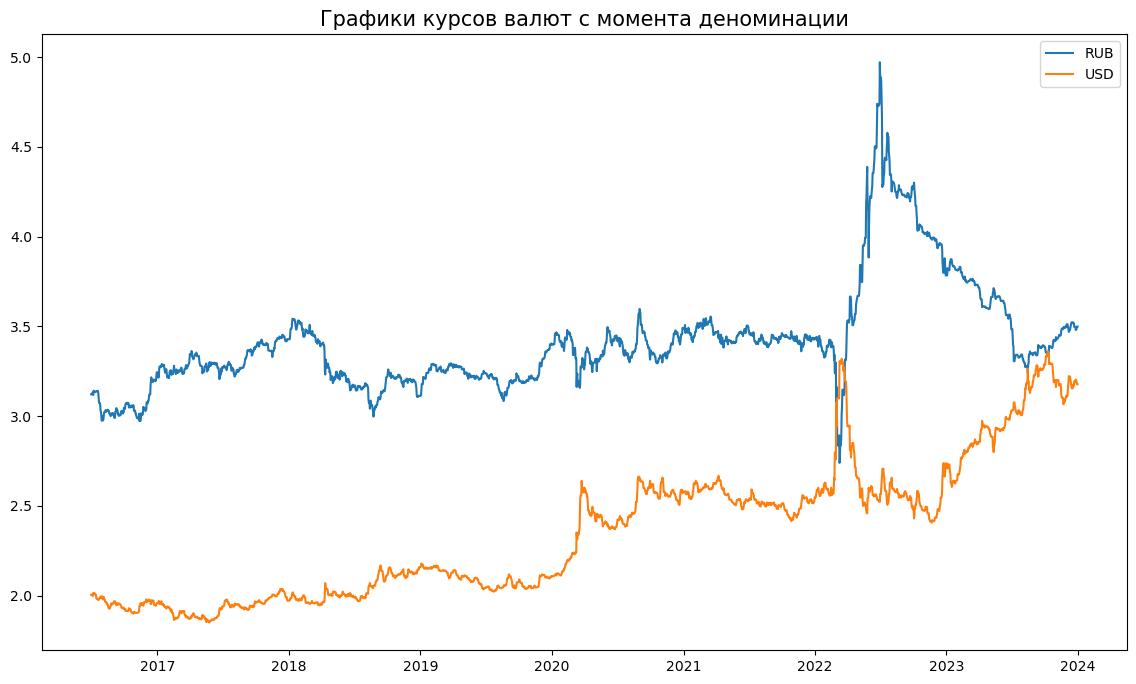
\includegraphics[scale=0.5]{images/img01}
		\caption{Временные ряды курсов валют по отношению к BYN}
		\label{fig:img01}
		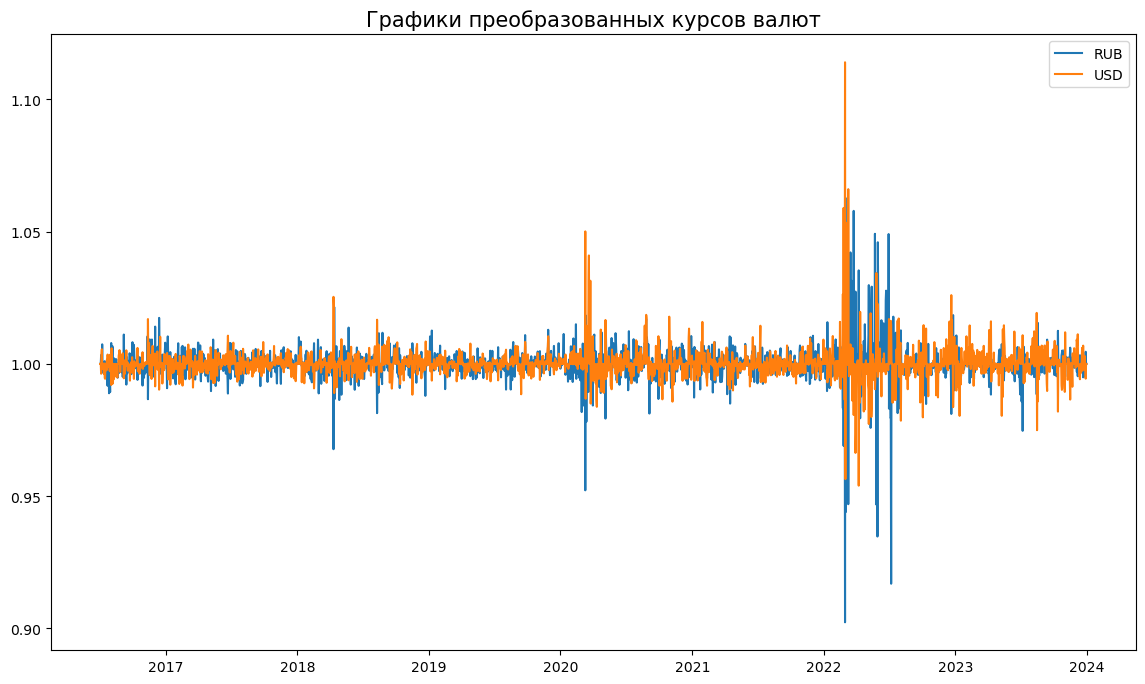
\includegraphics[scale=0.5]{images/img02}
		\caption{Временные ряды темпов роста курсов валют по отношению к BYN}
		\label{fig:img02}
	\end{figure}
	
	Рассмотрим временные ряды курсов показателей ИПЦ (Рис. 2).
	Выдвигаем гипотезу для каждого временного ряда
	$$H_0 : \{\text{временной ряд не стационарный}\},$$
	$$H_1 : \{\text{временной ряд стационарный}\}.$$
	Для каждого временного ряда с помощью теста Дики-Фуллера были оценены P-уровень значимости этой гипотезы. По результатам теста гипотеза $H_0$ отклоняется, а значит оба временных ряда уже являются стационарными (Таблица 1). 
	
	\begin{figure}[h]
		\centering
		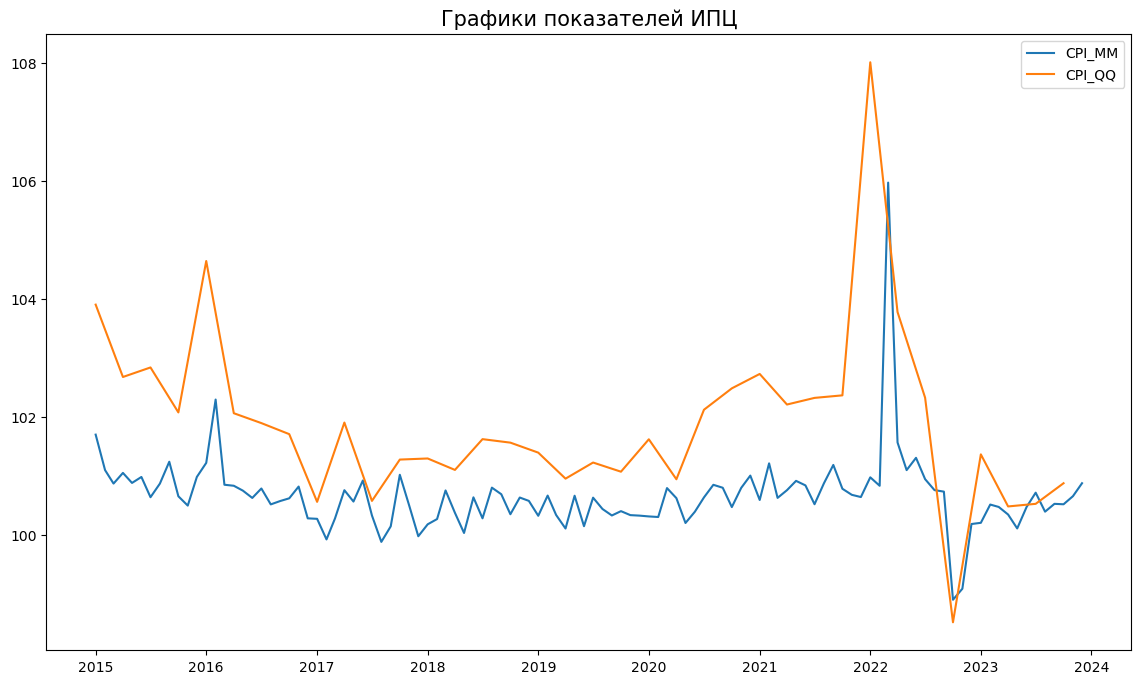
\includegraphics[scale=0.5]{images/img03}
		\caption{Временные ряды месячного и квартального показателей ИПЦ Беларуси}
		\label{fig:img03}
	\end{figure}
	
	
	\subsubsection{Предобработка эндогенных переменных}
	В качестве эндогенной переменной мы будем рассматривать показатель ВВП Беларуси. Исходный временной ряд обладает трендом, сезонностью, а также он не является стационарным. Поэтому сперва с помощью метода X13-ARIMA-SEATS (его подробное описание мы опустим) сделаем выделим сезонную составляющую из временного ряда. В итоге мы получим сезонно скорректированный временной ряд GDP\_SA (Рис. 3). Но получившийся временной ряд все также обладает трендом, поэтому мы проделаем преобразование, которое исключит тренд из временного ряда. Для этого мы можем взять новый временной ряд, который представляет собой натуральный логарифм исходного временного ряда:
	\begin{equation}
		GGDP\_RB\_SA_t^* = \ln\left(\dfrac{GGDP\_RB\_SA_t}{GGDP\_RB\_SA_{t-1}}\right).
	\end{equation}
	Для получившегося временного ряда с помощью теста Дики-Фуллера проверим гипотезу о нестационарности. По результатам тестирования (Таблица 1) гипотеза о нестационарности временного ряда отклоняется. Таким образом, полученный временной ряд будет стационарным.
	\begin{table}[]
		\centering
		\caption{ADF Statistic and p-value}
		\label{tab:adf_pvalue}
		\begin{tabular}{|c|c|c|}
			\hline
			Variable   & ADF Statistic & p-value        \\ \hline
			USD$^*$       & -13.789392   & $8.985260 \times 10^{-26}$ \\
			RUB$^*$      & -10.677356   & $4.021868 \times 10^{-19}$ \\
			CPI\_MM    & -4.834745    & $4.664619 \times 10^{-5}$  \\
			CPI\_QQ    & -4.031031    & $1.256461 \times 10^{-3}$  \\
			GGDP\_RB\_SA$^*$ & -6.825192  & $1.955999 \times 10^{-9}$  \\ \hline
		\end{tabular}
	\end{table}
	\newpage
	\begin{figure}[h]
		\centering
		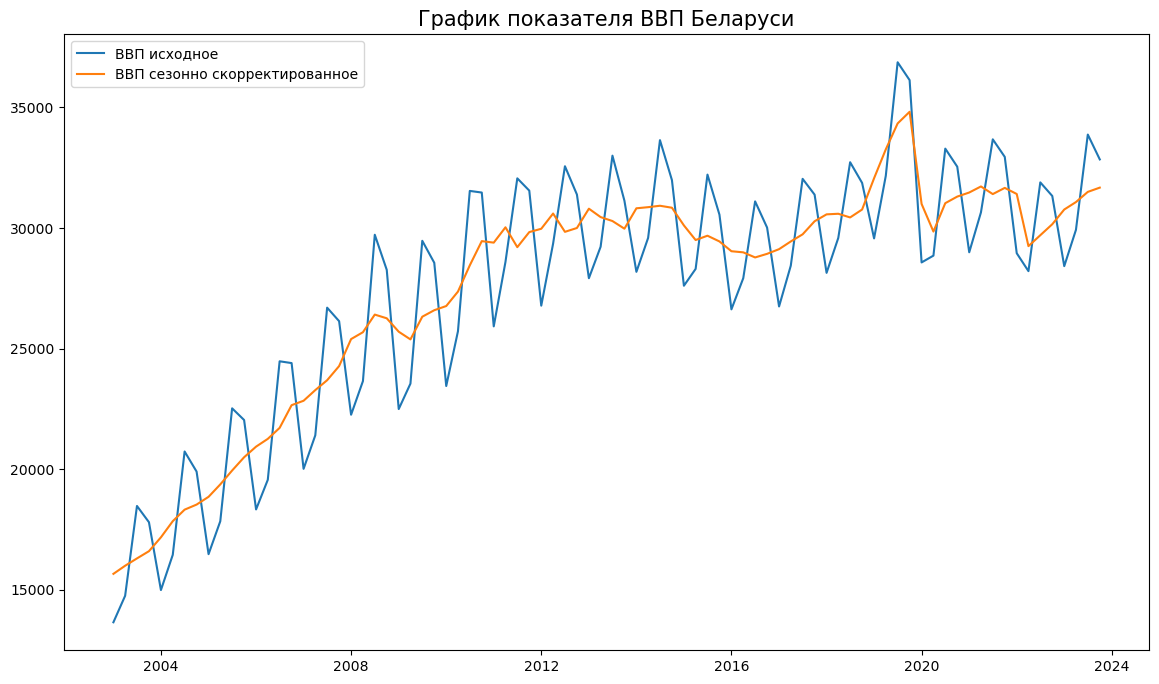
\includegraphics[scale=0.5]{images/img04}
		\caption{Графики исходного и сезонно скорректированного показателей ВВП Беларуси}
		\label{fig:img04}
		\centering
		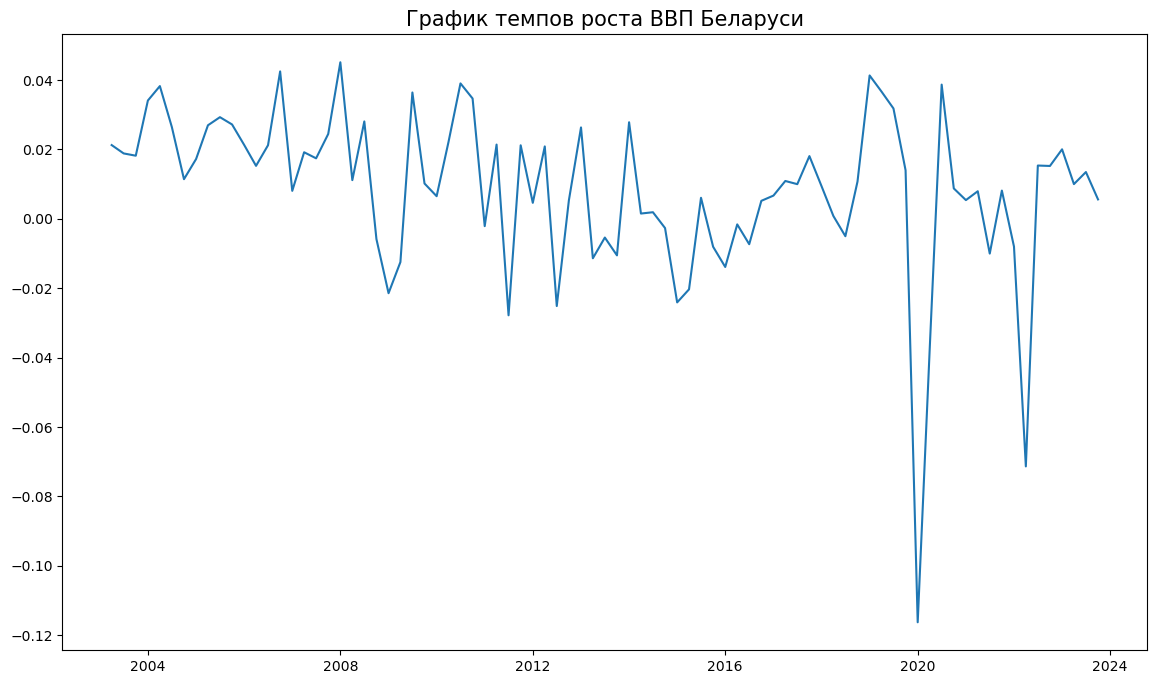
\includegraphics[scale=0.5]{images/img05}
		\caption{График темпов роста ВВП Беларуси}
		\label{fig:img05}
	\end{figure}
	
	
	\subsection{Построение квартальных моделей MIDAS по смешанным данным для реального ВВП Беларуси}
	
	Рассмотрение проведем для базовой модели MIDAS регрессии, введенной в пункте 1.3. В качестве примера мы возьмем библиотеку для Python под названием 'midas\_pro', в которой уже реализована базовая модель MIDAS, поддерживающая экспоненциальные лаги Алмон (1.3.5) и бета лаги (1.3.6).
	
	В качестве экзогенной переменной мы сначала возьмем только показатель ИПЦ месячной частоты, а затем попробуем добавить темпы роста одного из курсов валют.
	
	Как раньше было оговорено в пункте 1.12 в наукастинге мы не учитываем информацию о последнем доступном квартале при обучении модели. А сами модели мы сравниваем по последним 12 точкам. В данном случае мы имеем данные до 4 квартала 2023 года включительно, поэтому временные рамки, в которых будет проводиться ретроспективное сравнение моделей от 01.07.2020 до 01.07.2023, а последнее квартальное значение 01.10.2023 модели будут прогнозировать. 
	
	Сравнение моделей по ретроспективным прогнозам будет производиться по трем указанным в пункте 1.12 метрикам. По этим же метрикам будут оцениваться и будущие прогнозы моделей.
	
	Для всех MIDAS моделей выбиралось количество лагов для ежедневной экзогенной переменной равное 89, а для месячной экзогенной переменной 2. Таким образом, на значение ВВП в исследуемом квартале будут влиять значения курса в этом квартале и значения показателя ИПЦ в этом квартале.
	
	На Рис. 6 представлены ретроспективные прогнозы всех моделей MIDAS за на указанном временном промежутке.
	\begin{figure}[h]
		\centering
		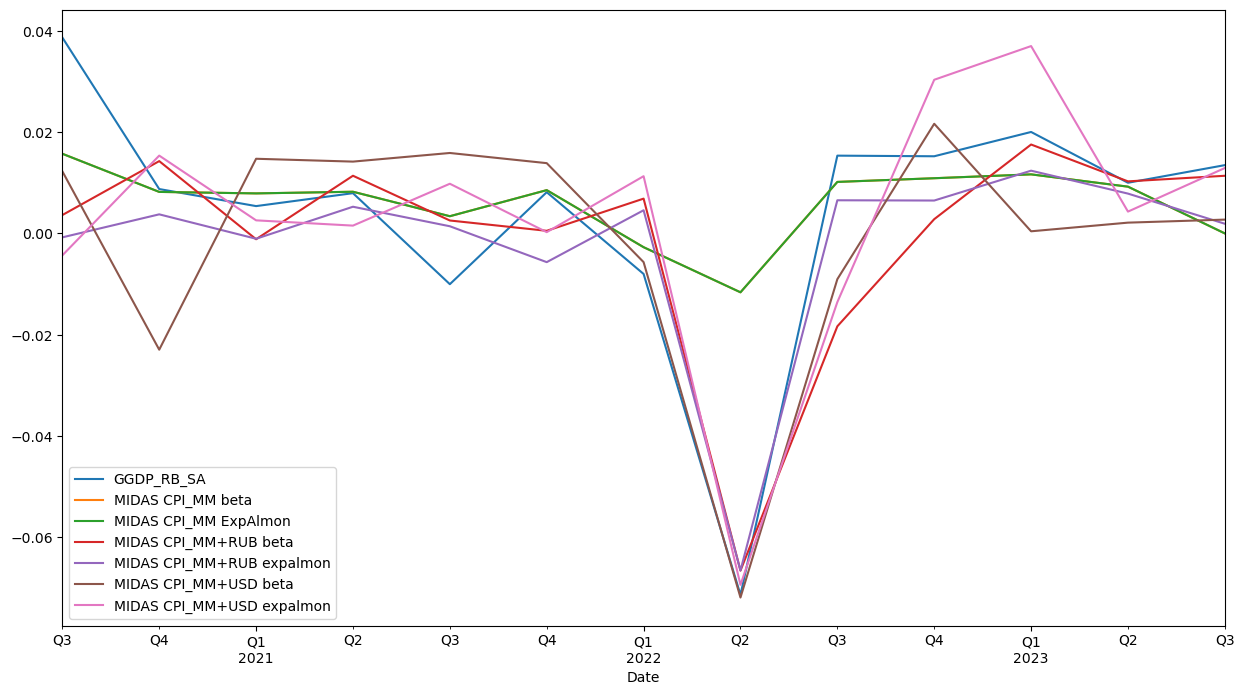
\includegraphics[scale=0.5]{images/img06}
		\caption{Графики ретроспективных прогнозов MIDAS моделей}
		\label{fig:img06}
	\end{figure}
	
	В таблице 2 представлены все оценки моделей на ретроспективных прогнозах.
\begin{table}[h]
	\centering
	\caption{Retrospective Evaluation Metrics}
	\label{tab:evaluation_metrics}
	\begin{tabular}{|c|c|c|c|}
		\hline
		Model & MAE & MAPE & RMSE \\
		\hline
		MIDAS CPI\_MM Beta          & 0.010561 & 0.473983 & 0.018825 \\
		MIDAS CPI\_MM ExpAlmon      & 0.010561 & 0.473978 & 0.018825 \\
		MIDAS CPI\_MM+RUB Beta      & 0.010875 & 0.816500 & 0.015378 \\
		MIDAS CPI\_MM+RUB ExpAlmon  & 0.010394 & 0.784645 & 0.013824 \\
		MIDAS CPI\_MM+USD Beta      & 0.013635 & 1.152350 & 0.016956 \\
		MIDAS CPI\_MM+USD ExpAlmon  & 0.013467 & 0.993322 & 0.017887 \\
		\hline
	\end{tabular}
\end{table}

	На основании полученной таблицы оценок можно сделать вывод, что наиболее оптимальной по всем оценкам оказалась модель MIDAS с эндогенными переменными CPI\_MM и RUB, использующая экспоненциальные лаги Алмон.
	
	Рассмотрим также и таблицу оценок для будущего прогноза (Таблица 3).
	
	\begin{table}[htbp]
		\centering
		\caption{Future Evaluation Metrics}
		\label{tab:evaluation_metrics}
		\begin{tabular}{|c|c|c|c|}
			\hline
			Model & MAE & MAPE & RMSE \\
			\hline
			MIDAS CPI\_MM Beta          & 0.004407 & 0.787724 & 0.004407 \\
			MIDAS CPI\_MM ExpAlmon      & 0.004407 & 0.787740 & 0.004407 \\
			MIDAS CPI\_MM+RUB Beta      & 0.001626 & 0.290612 & 0.006263 \\
			MIDAS CPI\_MM+RUB ExpAlmon  & 0.001587 & 0.283747 & 0.006301 \\
			MIDAS CPI\_MM+USD Beta      & 0.004614 & 0.824704 & 0.012502 \\
			MIDAS CPI\_MM+USD ExpAlmon  & 0.002240 & 0.400436 & 0.005648 \\
			\hline
		\end{tabular}
	\end{table}
	
	В ситуации с оценками для будущего прогноза также себя лучше всего показала модель MIDAS с экзогенными переменными CPI\_MM и RUB.
	
	На графике построенный будущий прогноз имеет вид (Рис. 7)
	\begin{figure}[h]
		\centering
		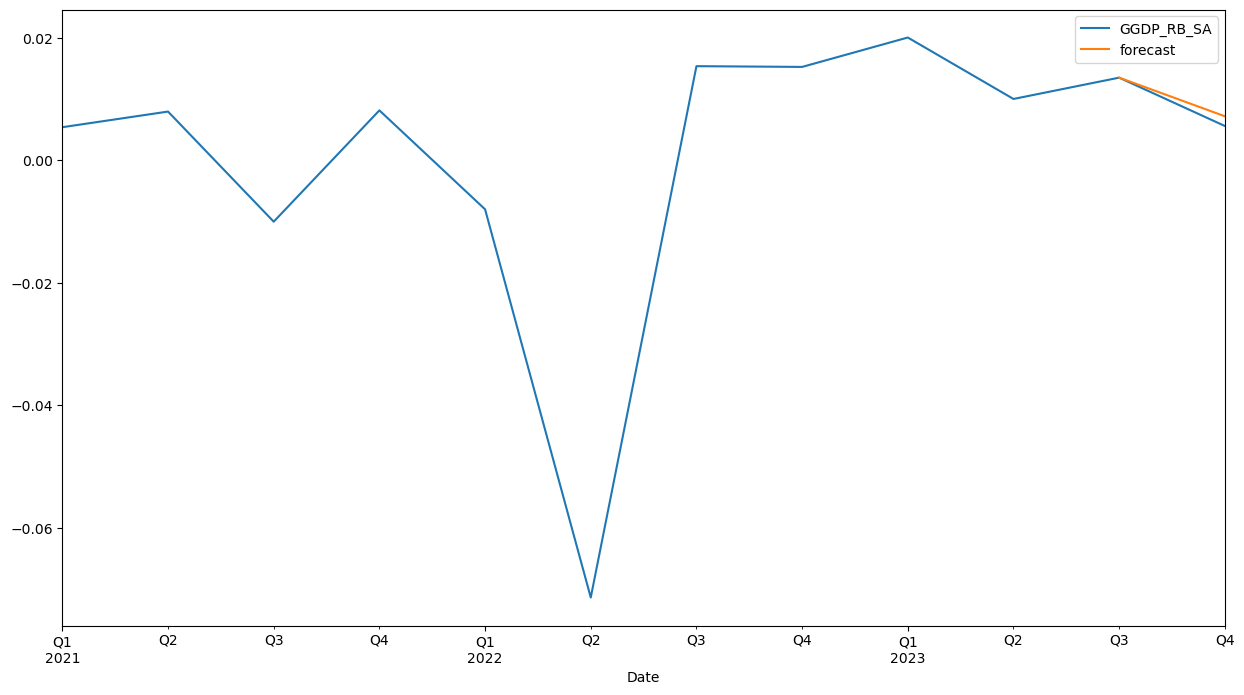
\includegraphics[scale=0.5]{images/img07}
		\caption{График будущего прогноза модели MIDAS для CPI\_MM + RUB}
		\label{fig:img07}
	\end{figure}
	
	\subsection{Построение квартальных моделей DL и ARDL по агрегированным данным для реального ВВП Беларуси}
	Для сравнения с MIDAS моделями построим также модели с распределенным запаздыванием. Ранее мы рассматривали DL-модель в пункте 1.2 и ARDL-модель в пункте 1.6. Сейчас же мы на практике построим эти модели и сравним результаты их оценок с предыдущими моделями.
	
	Как ранее было сказано, DL-модели могут работать лишь с данными находящимися на одной частоте. Поэтому в качестве эндогенной переменной мы возьмем квартальный ВВП Беларуси, а в качестве экзогенной переменной -- квартальный показатель ИПЦ Беларуси. 
	
	В данном случае у нас имеется временной ряд квартальных значений показателя ИПЦ. Однако такое бывает не всегда, вследствие чего приходится производить агрегацию данных более высокой частоты к данным более низкой частоты. Одним из вариантов в данном случае мог быть выбор в качестве квартального значения ИПЦ значение, полученное в последнем месяце этого квартала.
	
	Положим число лагов для $x_t$ равное 1 в моделях DL и ARDL, а число лагов для $y_t$ равное 4 в модели ARDL (по результатам проверки эти значения лагов являются оптимальными). 
	
	Чтобы мы могли сравнить DL-модели с MIDAS-моделями, мы также будем производить оценку рестроспективного прогноза по последним 12 точкам. Графики ретроспективного прогноза моделей изображены на Рис. 8.
	
	\begin{figure}[h]
		\centering
		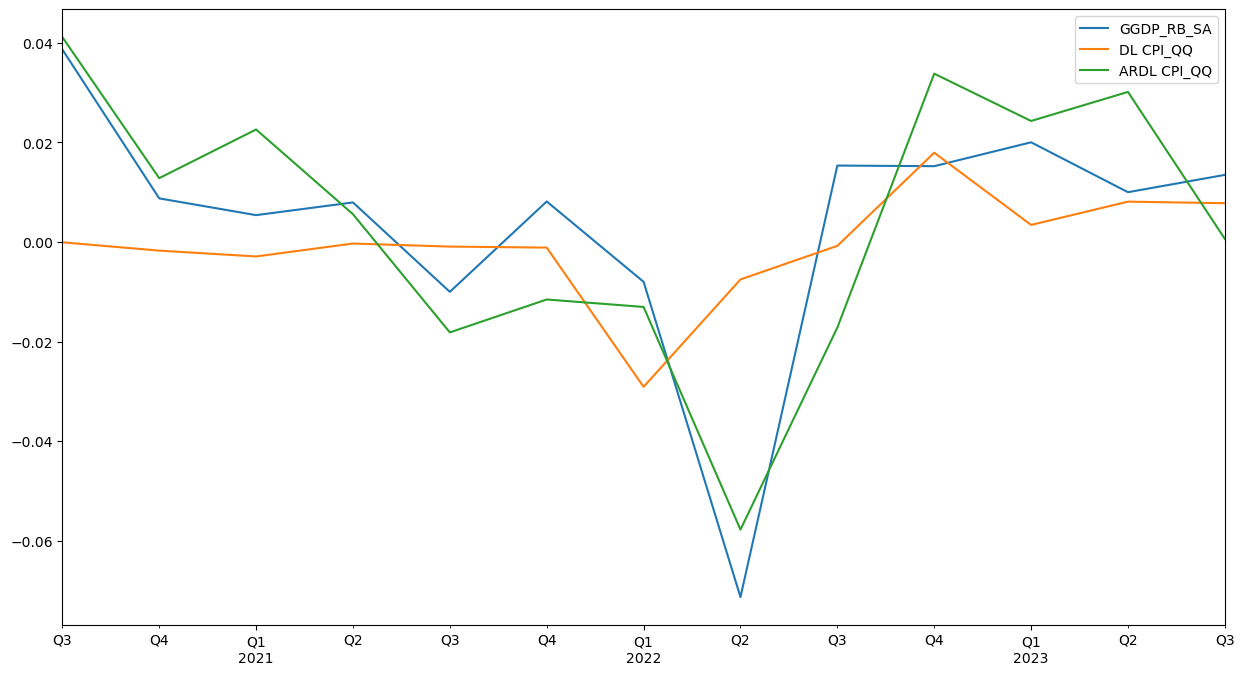
\includegraphics[scale=0.5]{images/img08}
		\caption{Графики ретроспективного прогноза DL и ARDL моделей}
		\label{fig:img08}
	\end{figure}
	
	\subsection{Сравнение лучшей MIDAS модели с DL моделями}
	Мы возьмем модель MIDAS с экзогенными переменными CPI\_MM и RUB и с экспоненциальными лагами Алмон и сравним ее с построенными  моделями с распределенным запаздыванием. Графики ретроспективных прогнозов изображены на Рис. 9, а результаты оценок этих прогнозов отображены в таблице 4.
	
	\begin{table}[htbp]
		\centering
		\caption{Evaluation Metrics}
		\label{tab:evaluation_metrics}
		\begin{tabular}{|c|c|c|c|}
			\hline
			Model & MAE & MAPE & RMSE \\
			\hline
			MIDAS CPI\_MM+RUB ExpAlmon & 0.013467 & 0.993322 & 0.017887 \\
			DL CPI\_QQ                 & 0.016318 & 1.001932 & 0.023231 \\
			ARDL CPI\_QQ               & 0.012386 & 1.122417 & 0.015147 \\
			\hline
		\end{tabular}
	\end{table}
	
	Таким образом, модель ARDL имеет также достаточно хорошие показатели оценок относительно модели MIDAS. А значит, если у нас имеются данные на одной частоте, то вполне оправдано будет использование модели ARDL. Но все же для задачи по смешанным данным модель ARDL будет не так эффективна как модель MIDAS, поскольку стоит учитывать тот факт, что агрегированные данные нам были заданы и нам не пришлось столкнуться с проблемами связанными с агрегацией данных более высокой частоты.
	\newpage
	
	\begin{figure}[h]
		\centering
		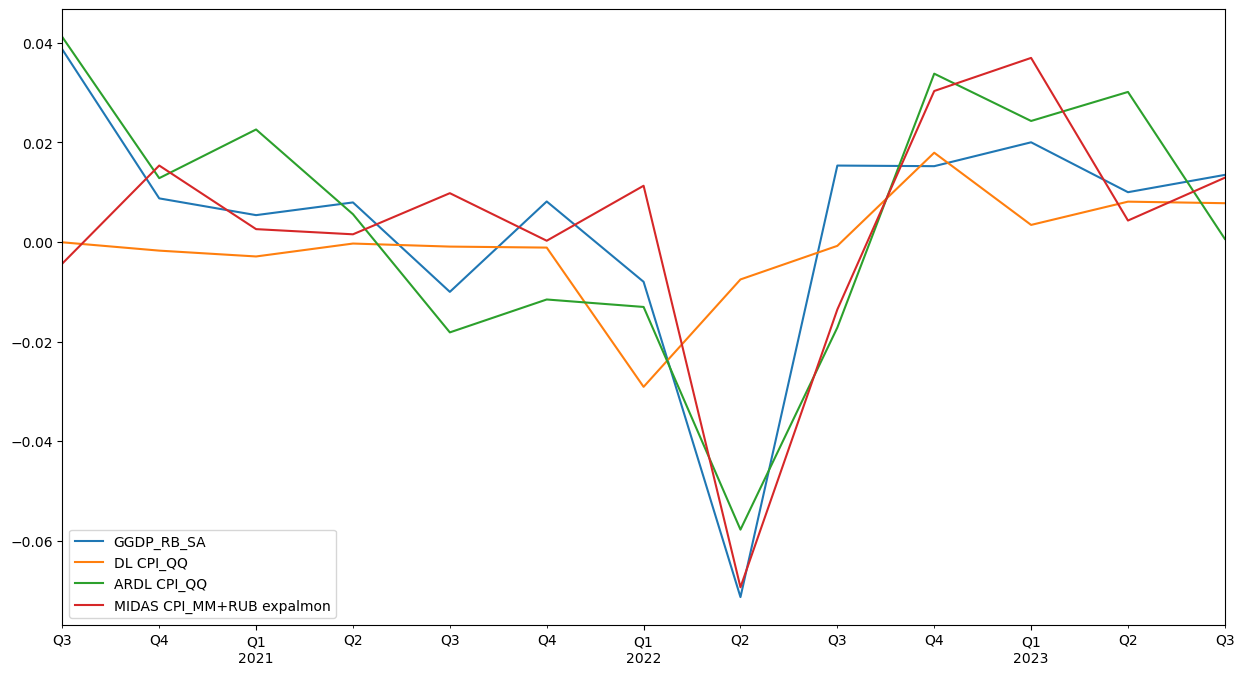
\includegraphics[scale=0.5]{images/img09}
		\caption{Графики ретроспективных прогнозов MIDAS, DL и ARDL моделей}
		\label{fig:img09}
	\end{figure}
	 
	
	\newpage
	\section*{ЗАКЛЮЧЕНИЕ}\addcontentsline{toc}{section}{ЗАКЛЮЧЕНИЕ}
	В данной курсовой работе мы рассмотрели такую задачу, как предсказывание временных рядом по данными разной частоты, и основные модели, решающие эту задачу. Мы также провели практические исследования модели MIDAS регрессии, которая является одной из основных моделей, применяемых в наукастинге.
	
	На сегодняшний день задача предсказания временных рядов по данным разной частоты остается все еще актуальной, так как мы на практическом примере убедились, что с помощью моделей, способных решать подобную задачу, мы можем прогнозировать значения такого важного макроэкономического показателя как ИПЦ.
	
	Нами были рассмотрены различные модели, работающие с данными разной частоты. Подытоживая, мы можем выделить три основных типа моделей (в зависимости от используемых этими моделями подходов):
	\begin{itemize}
		\item модели MIDAS регрессии;
		\item модели векторной авторегрессии;
		\item динамические факторные модели.
	\end{itemize}
	Все эти модели хорошо себя показывают в прогнозировании временных рядов со смешанными частотами. Выбор модели целиком зависит от поставленной задачи и проведенных исследований. Целесообразно для реальной задачи прогнозирования каких-либо показателей использовать все предложенные модели, чтобы выявить лучший прогноз. Так как для каждой задачи какая-то конкретная модель может показать себя лучше остальных. Проблемой может выступать лишь то, что эти модели реализованы в относительно небольшом числе пакетов, что может затруднять процесс исследований.
	
	Нами также были рассмотрены основные критерии, применяемые для оценки качества прогнозов моделей. Но на практике выбор критерия также зависит непосредственно от данных. Как и с моделями, целесообразнее будет использовать сразу несколько различных оценок качества прогнозов и стараться минимизировать, если и не все, то большинство этих оценок.
	
	Во второй главе нами были проведены практические исследования с использованием модели MIDAS регрессии для предсказания реальных временных рядов:
	\begin{itemize}
		\item были исследованы статистические свойства временных рядов ВВП, ИПЦ и курсов валют;
		\item были построены модели MIDAS регрессии и модели с распределенным запаздыванием;
		\item была проведена оценка точности ретроспективных и будущих прогнозов для моделей MIDAS регрессии.
	\end{itemize} 
	Исходя из проведенных исследований, можем заключить, что, используя модель MIDAS регрессии, мы можем исследовать зависимость между переменными более низкой частоты и переменными более высокой частоты. Любые эконометрические модели не позволят с точностью прогнозировать будущие значения, однако они позволяют выделять зависимость между переменными там, где она есть.
	
	Проведенные нами исследования позволяют нам также сделать выводы о существовании взаимосвязи между ВВП Беларуси и показателями ИПЦ и курсом валют.
	\newpage
	\section*{СПИСОК ИСТОЧНИКОВ}\addcontentsline{toc}{section}{СПИСОК ИСТОЧНИКОВ}
	\begin{enumerate}
		\item Foroni, C. A survey of econometric methods for mixed frequency data / C. Foroni, M. Marcellino // Working Paper 2013/06, Norges Bank.
		\item Ghysels, E., Santa-Clara P., Valkanov R. 2002. The MIDAS touch: Mixed data sampling regression models, Working paper, UNC and UCLA.
		\item Макеева, Н.М., Наукастинг элементов использования ВВП России / Н.М. Макеева, И.П. Станкевич // Статья 2022/10, Экономический журнал ВШЭ.
		\item Foroni, C. Unrestricted Mixed Data Sampling (U-MIDAS): MIDAS Regressions With Unrestricted Lag Polynomials / C. Foroni, M. Marcellino, C. Schumacher // Discussion paper 2015, Deutsche Bundesbank.
		\item Станкевич И.П. Сравнение методов наукастинга макроэкономических индикаторов на примере российского ВВП // Прикладная эконометрика 2020. С. 113–127.
		\item Ghysels, E. Regression models with mixed sampling frequencies /  E. Andreou, A. Kourtellos // Journal of Econometrics 2010.
		\item Soybilgen, B. Nowcasting the New Turkish GDP / B. Soybilgen, E. Yazgan // Economics Bulletin, Volume 38, Issue 2, 
		С. 1083-1089
		\item Ghysels, E. MIDAS Regressions: Further Results and New Directions / E. Ghysels, A. Sinko, R. Valkanov // Working paper.
		\item Kuzin, V. MIDAS vs. Mixed-Frequency VAR:
		Nowcasting GDP in the Euro Area / V. Kuzin,
		M. Marcellino, C. Shumacher // EUI Working Paper.
		\item Харин, Ю. С. Теория вероятностей,
		математическая
		и прикладная статистика / Ю. С. Харин, Н. М. Зуев, Е. Е. Жук // Минск : БГУ, 2011. 
		\item Малюгин, В. Краткосрочное прогнозирование и наукастинг темпов роста инфляции на основе моделей по смешанным данным / В.И. Малюгин // Банкаўскі веснік. – 2024. – С. 1–13.
	\end{enumerate}
	\newpage
	\section*{ПРИЛОЖЕНИЕ}\addcontentsline{toc}{section}{ПРИЛОЖЕНИЕ}
	Полный листинг программы из главы 2:
	\begin{python}
		%matplotlib inline
		import matplotlib.pyplot as plt
		import seaborn as sns
		
		import numpy as np
		import pandas as pd
		
		import warnings
		import datetime
		
		import statsmodels.api as sm
		from statsmodels.tsa.x13 import x13_arima_analysis
		from statsmodels.tsa.stattools import adfuller
		from statsmodels.tsa.seasonal import seasonal_decompose
		import statsmodels.stats as sm_stat
		import statsmodels.tsa as smt
		import scipy.optimize as optimize
		import statsmodels.formula.api as smf
		from statsmodels.tsa.api import ARDL
		from sklearn.model_selection import train_test_split
		from statsmodels.tsa.ardl import ardl_select_order
		
		from itertools import product
		
		from sklearn.metrics import mean_squared_error, mean_absolute_error, mean_absolute_percentage_error
		
		
		from midas.mix import mix_freq, mix_freq2
		from midas.adl import estimate, forecast, midas_adl, rmse, estimate2,forecast2, midas_adl2
		
		ex_rates = pd.read_csv('ex_rates_2024.csv', parse_dates=['Date'], dayfirst=False, index_col='Date', sep=',')['2016-07-01':'2023-12-31']
		
		growth_ex_rates = (ex_rates / ex_rates.shift()).dropna().rename(columns={'RUB' : 'GRUB', 'USD' : 'GUSD', 'EUR' : 'GEUR'})
		log_growth_ex_rates = np.log(growth_ex_rates)
		
		usd = adfuller(growth_ex_rates['GUSD'])
		rur = adfuller(growth_ex_rates['GRUB'])
		
		cpi_mm = pd.read_csv('cpi_mm_2023.csv', parse_dates=['Date'], dayfirst=True, index_col='Date', sep=',')
		cpi_qq = pd.read_csv('cpi_qq_2023.csv', parse_dates=['Date'], dayfirst=True, index_col='Date', sep=',')
		
		gdp = pd.read_csv('gdp_data_2023.csv', parse_dates=['Date'], dayfirst=True, date_format='%Y-%m-%d', index_col='Date', sep=',').dropna()['2003-01-01':]
		
		import os
		os.chdir(r'C:\Users\bzzdwn\Downloads\x13as_ascii-v1-1-b60\x13as')
		
		x13_analysis_gdp_rb = x13_arima_analysis(gdp.RB_GDP)
		print(x13_analysis_gdp_rb.stdout.decode("utf-8"))
		
		gdp_rb_sa = pd.DataFrame(x13_analysis_gdp_rb.seasadj).rename(columns={'seasadj' : 'GDP_RB_SA'})
		ggdp_rb_sa = np.log(gdp_rb_sa / gdp_rb_sa.shift()).dropna().rename(columns={'GDP_RB_SA' : 'GGDP_RB_SA'})
		
		DF_test = pd.DataFrame([[usd[0], rur[0], adfuller(cpi_mm)[0], adfuller(cpi_qq)[0], adfuller(ggdp_rb_sa)[0], adfuller(ggdp_ru_sa)[0]], 
		[usd[1], rur[1], adfuller(cpi_mm)[1], adfuller(cpi_qq)[1], adfuller(ggdp_rb_sa)[1], adfuller(ggdp_ru_sa)[1]]], 
		index=["ADF Statistic", "p-value:"], 
		columns=["GUSD", "GRUB", "CPI_MM", "CPI_QQ", "GGDP_RB_SA", "GGDP_RU_SA"]).T
		print(DF_test)
		
		
		models_predictions_statistics = pd.DataFrame(None, columns=['MAE', 'MAPE', 'RMSE'])
		models_forecast_statistics = pd.DataFrame(None, columns=['MAE', 'MAPE', 'RMSE'])
		
		y, yl, x, yf, ylf, xf = mix_freq(lf_data=ggdp_rb_sa.GGDP_RB_SA, 
		hf_data=cpi_mm.CPI_MM, 
		xlag=12,  
		ylag=1, 
		horizon=1,
		start_date=datetime.datetime(2003,1,1),
		end_date=datetime.datetime(2023,7,1))
		model_6 = estimate(y, yl, x, poly='beta')
		
		fc1 = forecast(x, yl, model_6, poly='beta')
		forecast1_df = fc1.join(ggdp_rb_sa.GGDP_RB_SA.loc['2020-07-01':'2023-07-01']).shift(-1).fillna(0)
		forecast1_df['residuals'] = forecast1_df.yfh - forecast1_df.GGDP_RB_SA
		
		models_predictions_statistics.loc['MIDAS CPI_MM Beta'] = [
		mean_absolute_error(ggdp_rb_sa.GGDP_RB_SA.loc['2020-07-01':'2023-07-01'], forecast1_df.yfh.loc['2020-07-01':'2023-07-01']),
		mean_absolute_percentage_error(ggdp_rb_sa.GGDP_RB_SA.loc['2020-07-01':'2023-07-01'], forecast1_df.yfh.loc['2020-07-01':'2023-07-01']),
		np.sqrt(mean_squared_error(ggdp_rb_sa.GGDP_RB_SA.loc['2020-07-01':'2023-07-01'], forecast1_df.yfh.loc['2020-07-01':'2023-07-01']))]
		
		models_results = pd.DataFrame(ggdp_rb_sa.GGDP_RB_SA.loc['2020-07-01':'2023-07-01'])
		models_results = pd.concat([models_results, forecast1_df.yfh.loc['2020-07-01':'2023-07-01']], axis=1).rename(columns={'yfh' : 'MIDAS CPI_MM beta'})
		
		models_results.plot(figsize=(15,8), style=['-', '-'])
		
		fc = forecast(xf, ylf, model_6, poly='beta')
		forecast_df = fc.join(yf)
		forecast_df['residuals'] = forecast_df.yfh - forecast_df.GGDP_RB_SA
		
		forecasting = ggdp_rb_sa.tail(2).head(1)
		forecasting = forecasting.join(forecast_df.yfh, how='outer')
		forecasting.iloc[0, 1] = forecasting.iloc[0, 0]
		forecasting=forecasting.drop(columns=['GGDP_RB_SA']).rename(columns={'yfh':'forecast'})
		
		models_forecast_statistics.loc['MIDAS CPI_MM Beta'] = [
		mean_absolute_error([ggdp_rb_sa.GGDP_RB_SA.loc['2023-10-01']], forecast_df.yfh),
		mean_absolute_percentage_error([ggdp_rb_sa.GGDP_RB_SA.loc['2023-10-01']], forecast_df.yfh),
		np.sqrt(mean_squared_error([ggdp_rb_sa.GGDP_RB_SA.loc['2023-10-01']], forecast_df.yfh))]
		
		df_gdp = pd.concat([ggdp_rb_sa.GGDP_RB_SA['2021-01-01':'2023-10-01'], 
		forecasting, ], axis=1)
		df_gdp.plot(figsize=(15,8), style=['-', '-'])
		
		def lag(x, n):
		if n == 0:
		return x
		if isinstance(x, pd.Series):
		return x.shift(n) 
		else:
		x = pd.Series(x)
		return x.shift(n) 
		
		x = x.copy()
		x[n:] = x[0:-n]
		x[:n] = np.nan
		return x
		
		lags = 1
		endog = ggdp_rb_sa.GGDP_RB_SA['2015-01-01':'2023-07-01']
		exog = cpi_qq.CPI_QQ['2015-01-01':'2023-07-01']
		
		X = np.zeros((exog.shape[0], lags+1))
		for i in range(lags + 1):
		X[:,i] = lag(exog, i).fillna(0)
		X = sm.add_constant(X)
		model = sm.OLS(endog.values, X).fit()
		print(model.summary())
		
		dl_predicts = model.predict(exog=pd.DataFrame(X).set_index(exog.index))
		models_results = pd.DataFrame(ggdp_rb_sa.GGDP_RB_SA.loc['2020-07-01':'2023-07-01'])
		
		models_predictions_statistics.loc['DL CPI_QQ'] = [
		mean_absolute_error(ggdp_rb_sa.GGDP_RB_SA.loc['2020-07-01':'2023-07-01'], dl_predicts.loc['2020-07-01':'2023-07-01']),
		mean_absolute_percentage_error(ggdp_rb_sa.GGDP_RB_SA.loc['2020-07-01':'2023-07-01'], dl_predicts.loc['2020-07-01':'2023-07-01']),
		np.sqrt(mean_squared_error(ggdp_rb_sa.GGDP_RB_SA.loc['2020-07-01':'2023-07-01'], dl_predicts.loc['2020-07-01':'2023-07-01']))]
		
		models_results = pd.concat([models_results, dl_predicts.loc['2020-07-01':'2023-07-01']], axis=1).rename(columns={0 : 'DL CPI_QQ'})
		models_results.plot(figsize=(15,8), style=['-', '-'])
		
		ardl = ardl_select_order(
		endog, 6, pd.DataFrame(exog), 6, ic="aic", trend="ct"
		)
		print(f"The optimal order is: {ardl.model.ardl_order}")
		ardl_model = ardl.model.fit()
		print(ardl_model.summary())
		
		ardl_predicts = ardl_model.predict(exog=pd.DataFrame(exog))
		
		models_predictions_statistics.loc['ARDL CPI_QQ'] = [
		mean_absolute_error(ggdp_rb_sa.GGDP_RB_SA.loc['2020-07-01':'2023-07-01'], ardl_predicts.loc['2020-07-01':'2023-07-01']),
		mean_absolute_percentage_error(ggdp_rb_sa.GGDP_RB_SA.loc['2020-07-01':'2023-07-01'], ardl_predicts.loc['2020-07-01':'2023-07-01']),
		np.sqrt(mean_squared_error(ggdp_rb_sa.GGDP_RB_SA.loc['2020-07-01':'2023-07-01'], ardl_predicts.loc['2020-07-01':'2023-07-01']))]
		
		models_results = pd.concat([models_results, ardl_predicts.loc['2020-07-01':'2023-07-01']], axis=1).rename(columns={0 : 'ARDL CPI_QQ'})
		models_results.plot(figsize=(15,8), style=['-', '-'])
		
		print(models_predictions_statistics)
		print(models_forecast_statistics)\end{python}
\end{document}